

 En este capítulo se comentará el proceso seguido para la realización de este proyecto detallando la planificación, diseño y el desarrollo del mismo estructurado en etapas.
 
\section{Seguimiento}

Una vez hecho el análisis, conocidos los objetivos que se quieren alcanzar en este proyecto y las herramientas que se utilizarán  empezaremos con la planificación del mismo.

Un punto muy  importante a tener en cuenta a la hora de realizar una planificación sería conocer los recursos y el tiempo del que disponemos.
Éste punto tan crucial se acentúa ya que este proyecto será realizado por una única persona lo que producirá sobrecargas en la planificación. Esto normalmente no es así ya que los proyectos se realizan por grupos de trabajos y muchas tareas pueden realizarse en paralelo disminuyendo apreciablemente la duración del proyecto.

Para realizar la planificación del proyecto hemos dividido el proyecto en tareas con unos objetivos bien marcados(Product Backlog). A su vez al seguir la metodología Scrum dividimos el proyecto en etapas(Sprint) de tiempo donde incluimos las tareas a realizar.
 En todas estas etapas incluimos los siguientes pasos:
 
 


\begin{itemize}
\item Definición del Sprint Backlog,  documento que recoge las tareas a realizar y quién las desempeña. En este caso al solo trabajar yo en el proyecto haré todas las tareas.


\item División del Sprint Backlog en tareas más sencillas y abordables (Backlog items). 



\item Diseño de cada una de las tareas del punto anterior.
\item  Implementacion de las tareas.
\item Pruebas.
\end{itemize}



\section{Duración  y costes}
 A continuación en la tabla siguiente se ha realizado una estimación de tiempos y de costes de este proyecto.
 Cuando se realiza una estimación de costes tenemos que tener en cuenta los gastos en material, licencias y los gastos propios. En mi caso los gastos de materias y de licencias es nulo ya que el material es el del alumno y licencias y gastos propios son nulos.
 En la siguiente tabla se detalla el esfuerzo horas-hombre de cada uno de los roles dentro del proyecto. 
 
 La jornada laboral sería de 5 horas y la duración de cada Sprint 20 días, lo que nos hace obtener el siguiente coste:


\begin{figure}[H]
		\centering
		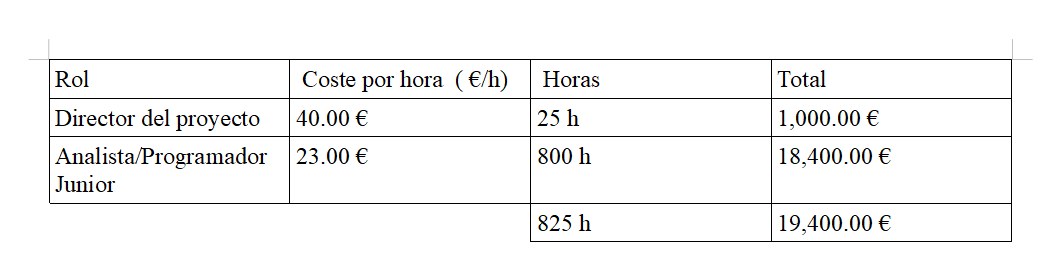
\includegraphics[width=0.75\textwidth] {coste.png}
		\caption{Costes asociados a este proyecto }
	\end{figure}






\begin{itemize}
\item En el rol de director de proyecto estarían los que 
supervisan y evalúan el proyecto. En este caso los directores realizarán este rol.

\item Analista/programador Junior, en este rol estaría la persona encargada de las tareas de análisis, diseño, desarrollo y de la creación de las pruebas para este proyecto. Al estar realizado por mi yo me encargaría de este rol.





\end{itemize}
\section{Sprints}

Como se comentó a lo largo de este capítulo la metodología usada será  Scrum y el proyecto será dividido en Sprints de 4 semanas cada uno. El número de Sprint que estimamos sería de 8.




 Antes de empezar con los Sprint comenzamos creando el Product Backlog. Ésto es una lista con todas las funcionalidades del la aplicación priorizadas de más a menos importancia para nuestro proyecto. 

\subsection{Sprint 1}

En este primer Sprint nos centraremos en las tareas relacionadas con la capa intermedia. Para ello comenzamos diseñando la base de datos y modelo de datos, algo fundamental en cualquier aplicación para no heredar carencias en capas superiores. Posteriormente los servicios necesarios para el servicio REST.


\subsection{Sprint 2}
 Una vez implementado el servicio Rest, el objetivo en este Sprint será hacer las pruebas para él.
 Una vez acabas las pruebas el siguiente paso dentro de esté Sprint será la creación de las maquetas que servirán para la capa de presentación/cliente, es decir, el interface del usuario. Estas maquetas se irán revisando y refinando a lo largo del proyecto.
 
\subsection{Sprint 3}

En este Sprint se comenzará con el desarrollo de la aplicación Android. Comenzaremos permitiendo que el usuario sea capaz que conocer su localización dentro del mapa y que al ir desplazándose cambie su ubicación como también obtener las coordenadas de su posición. Este punto será básico para el resto de la aplicación ya nos proporciona los datos necesarios para guardar puntos y rutas. La historia que se implementará será \textit{Gestión de puntos de interés (PDI)\textbf{•}}, los casos de uso realizados son los siguientes:

\begin{itemize}

\item\textbf{\textit{ R-PDI-1 Guardar Punto De Interés caza}}
\item\textit{ \textbf{R-PDI-2 Guardar Punto De Interés pesca}}
\item \textbf{\textit{R-PDI-3 Eliminar PDI}}
\item \textbf{\textit{R-PDI-4 Buscar los PDI}}
\end{itemize} 


\begin{figure}[htbp]
\begin{minipage}[b]{0.5\linewidth} %Una minipágina que cubre la mitad de la página
\centering
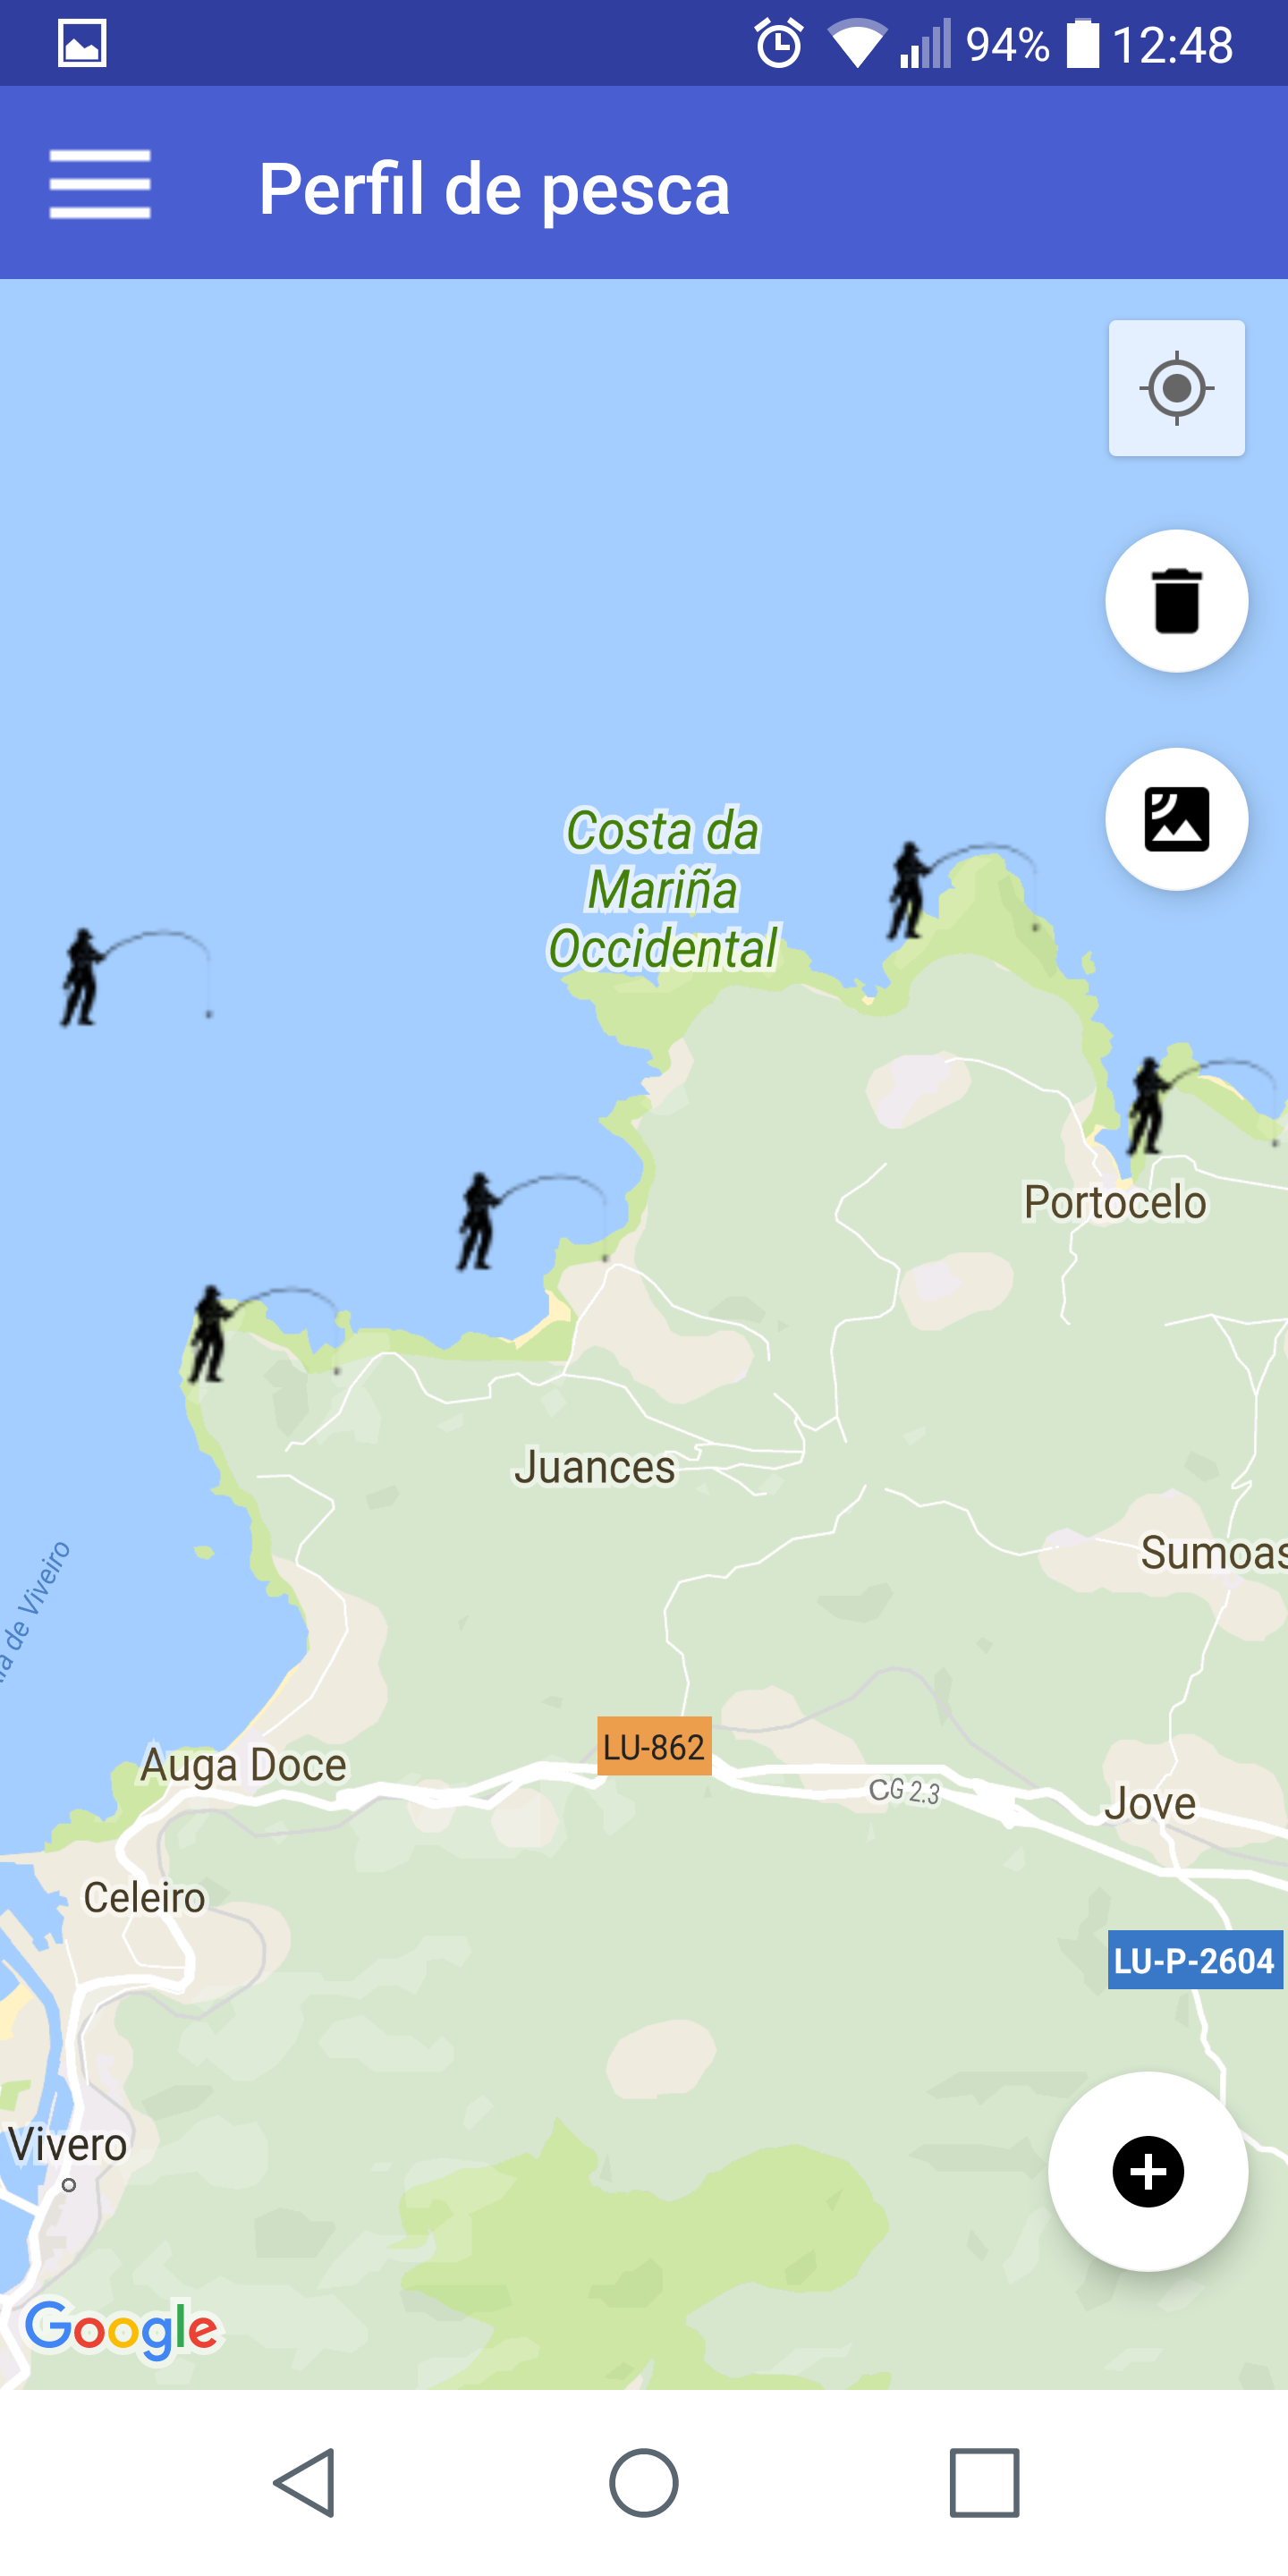
\includegraphics[width=6cm]{capturamovil/pdipesca.png}
 \label{figura1}
\caption{PDI pesca}

\end{minipage}
\hspace{0.5cm} % Si queremos tener un poco de espacio entre las dos figuras
\begin{minipage}[b]{0.5\linewidth}
\centering
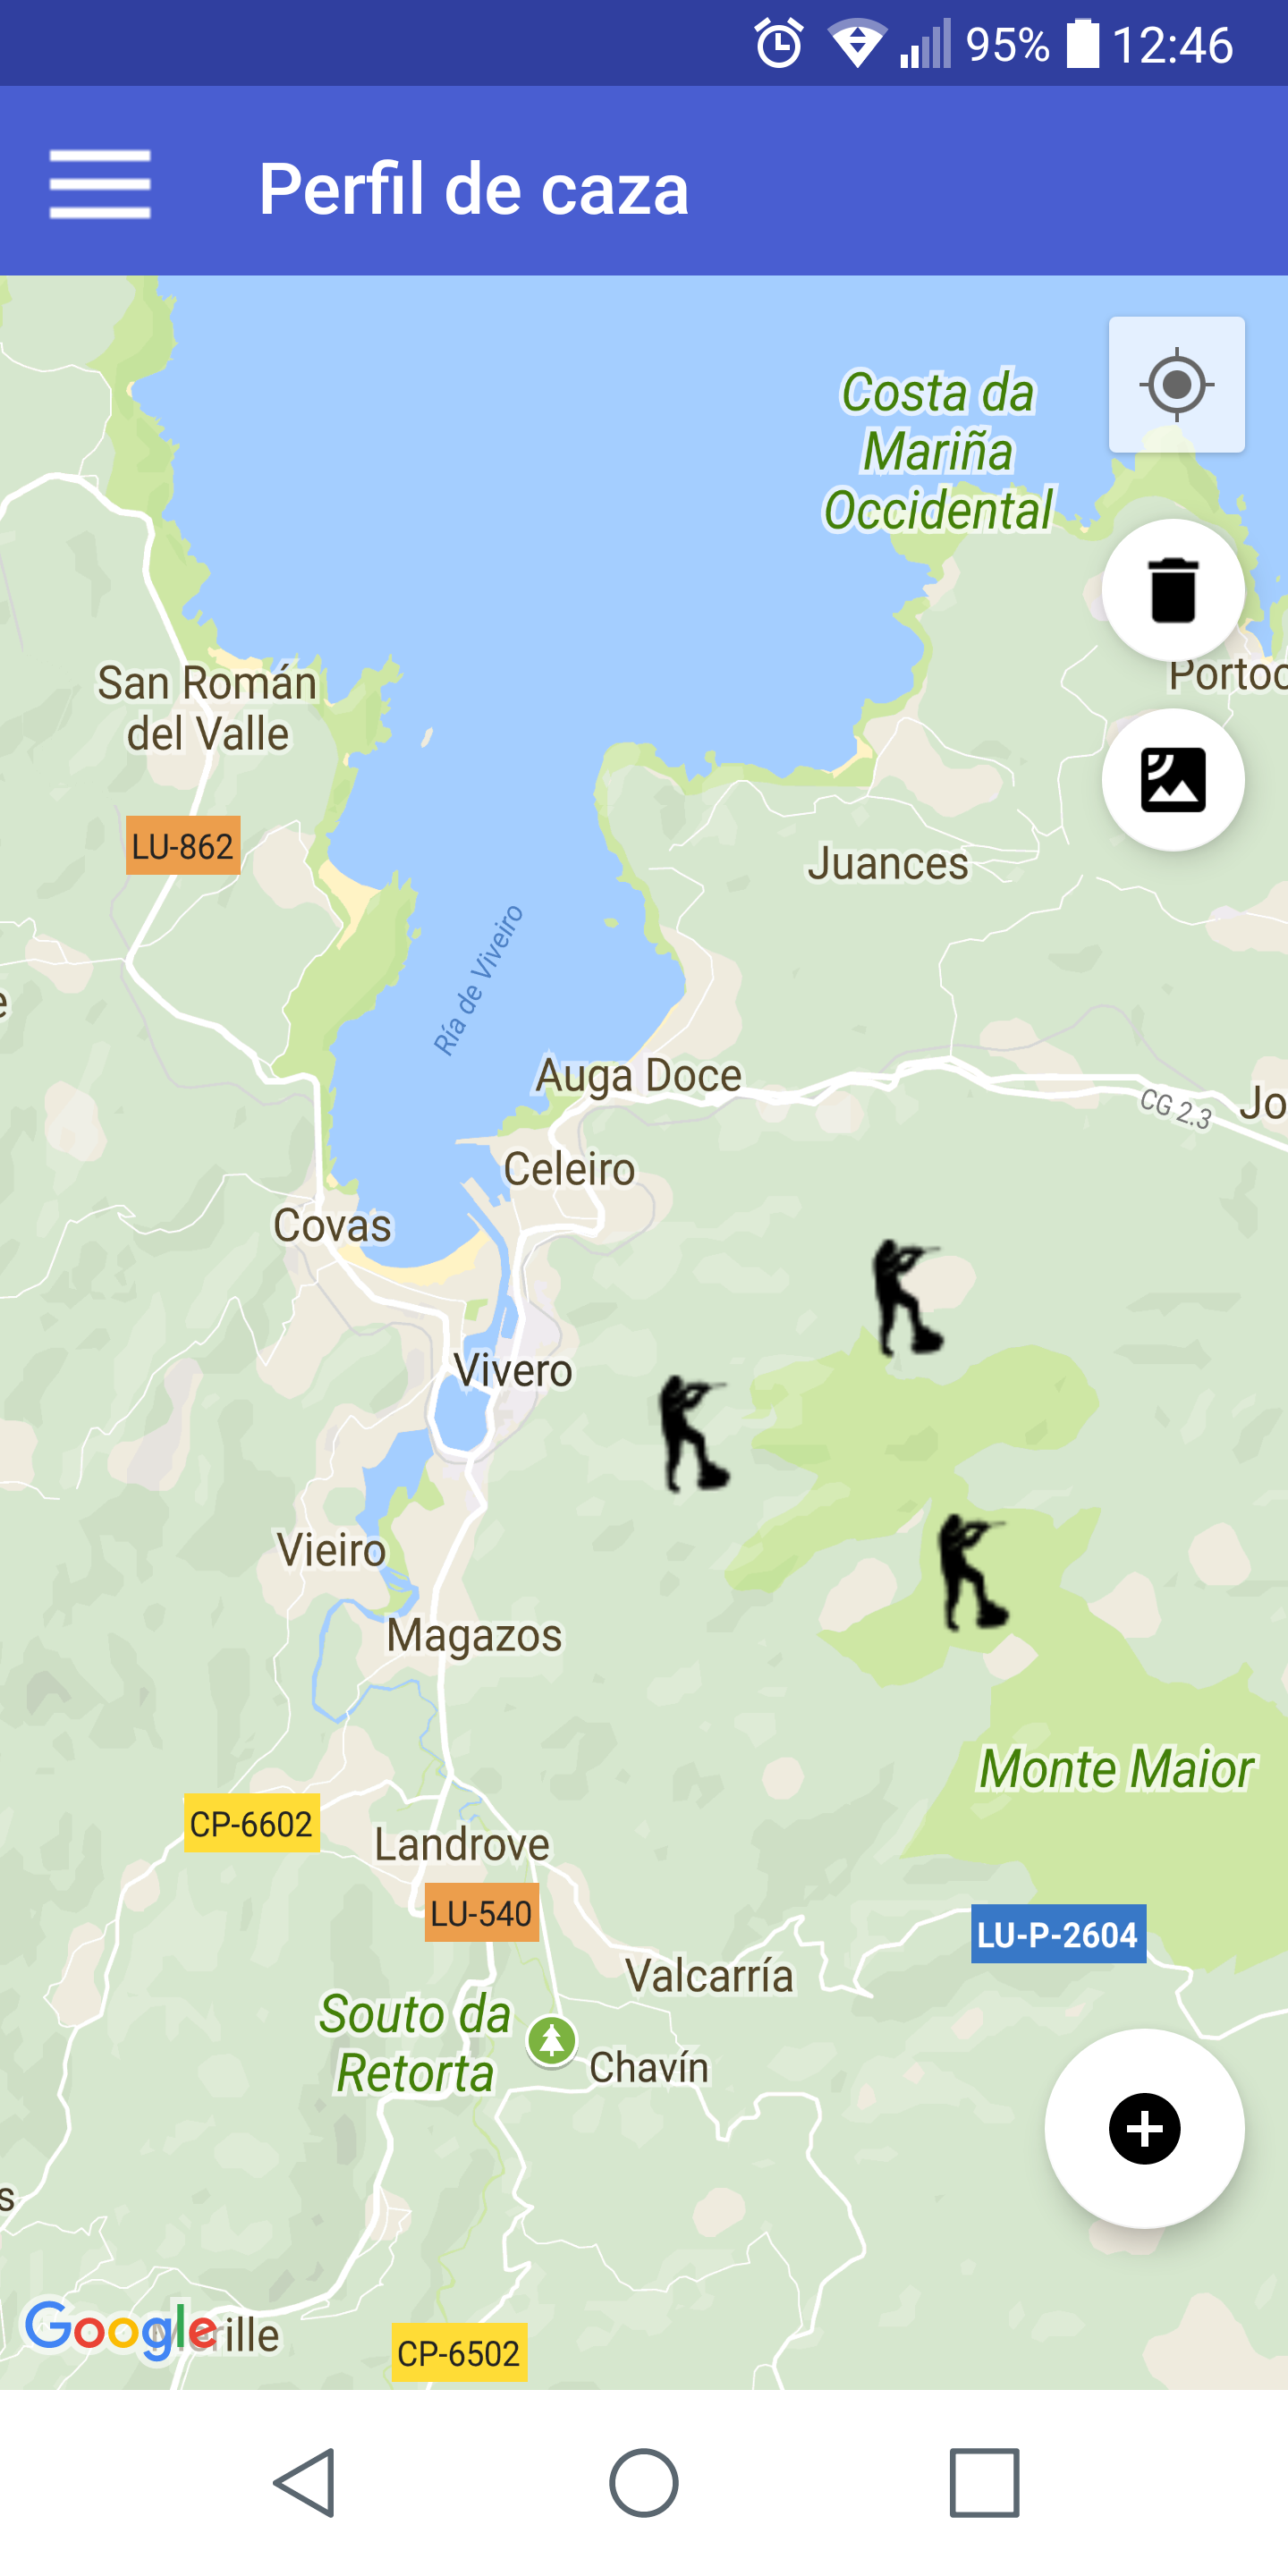
\includegraphics[width=6cm]{capturamovil/pdicaza.png}
 \label{figura2}
\caption{PDI caza}

\end{minipage}
\end{figure}



\begin{figure}[htbp]
\begin{minipage}[b]{0.5\linewidth} %Una minipágina que cubre la mitad de la página
\centering
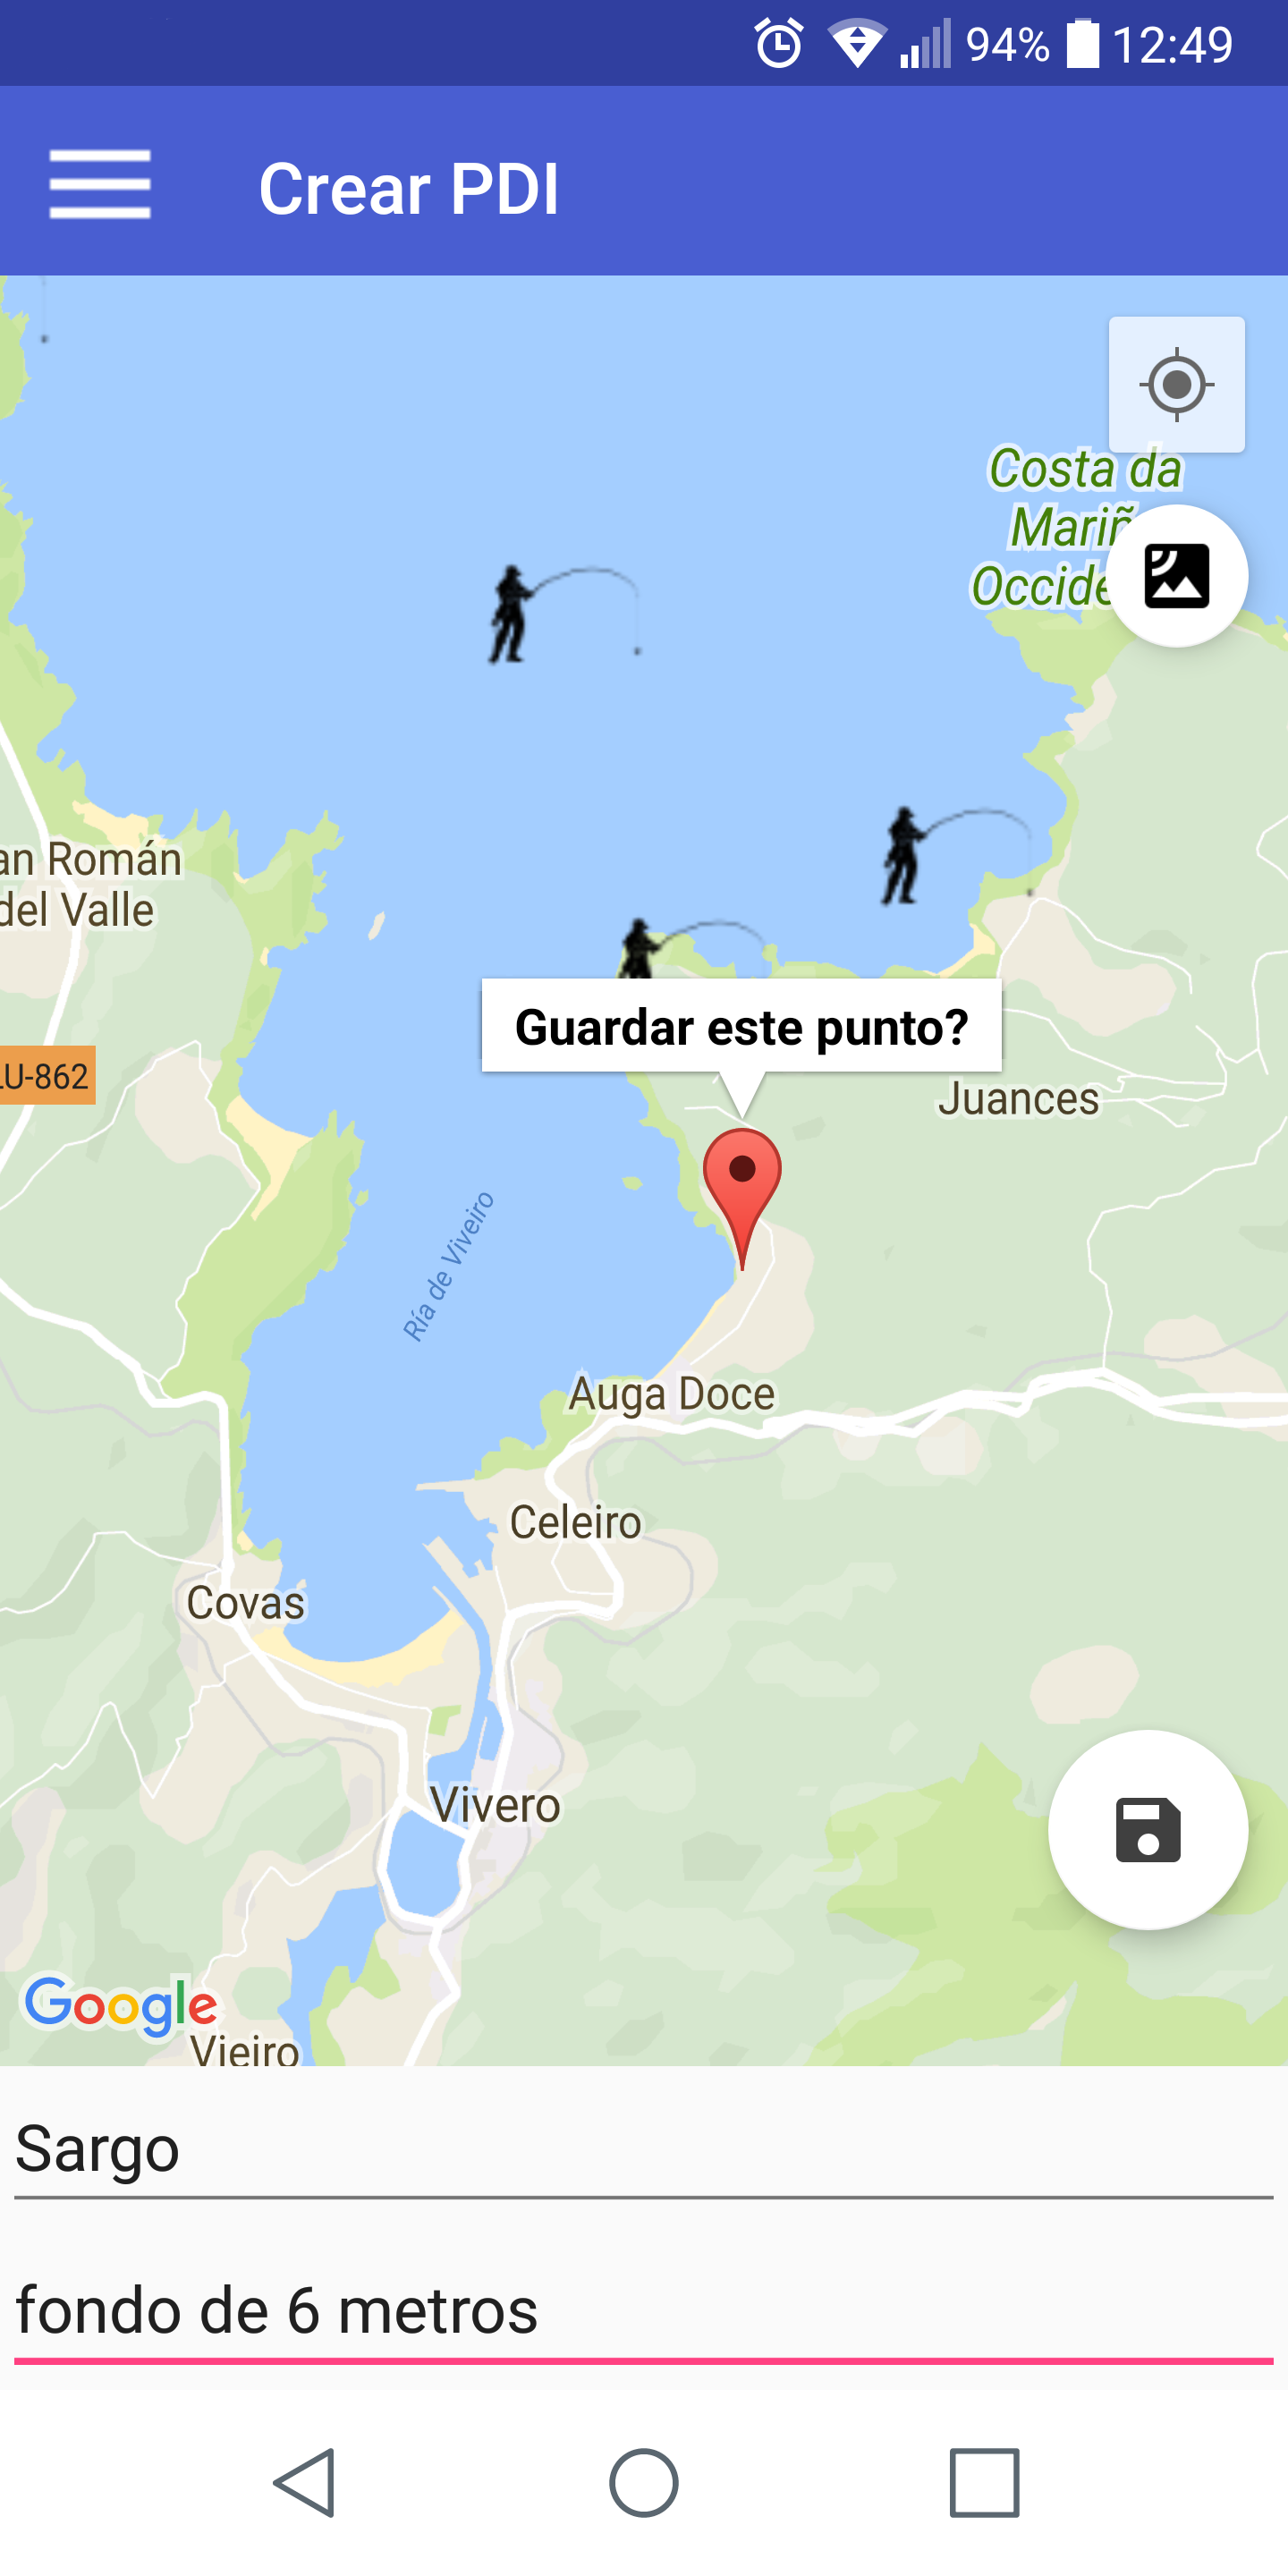
\includegraphics[width=6cm]{capturamovil/pdiguardar.png}
 \label{figura1}
\caption{Guardar PDI}

\end{minipage}
\hspace{0.5cm} % Si queremos tener un poco de espacio entre las dos figuras
\begin{minipage}[b]{0.5\linewidth}
\centering
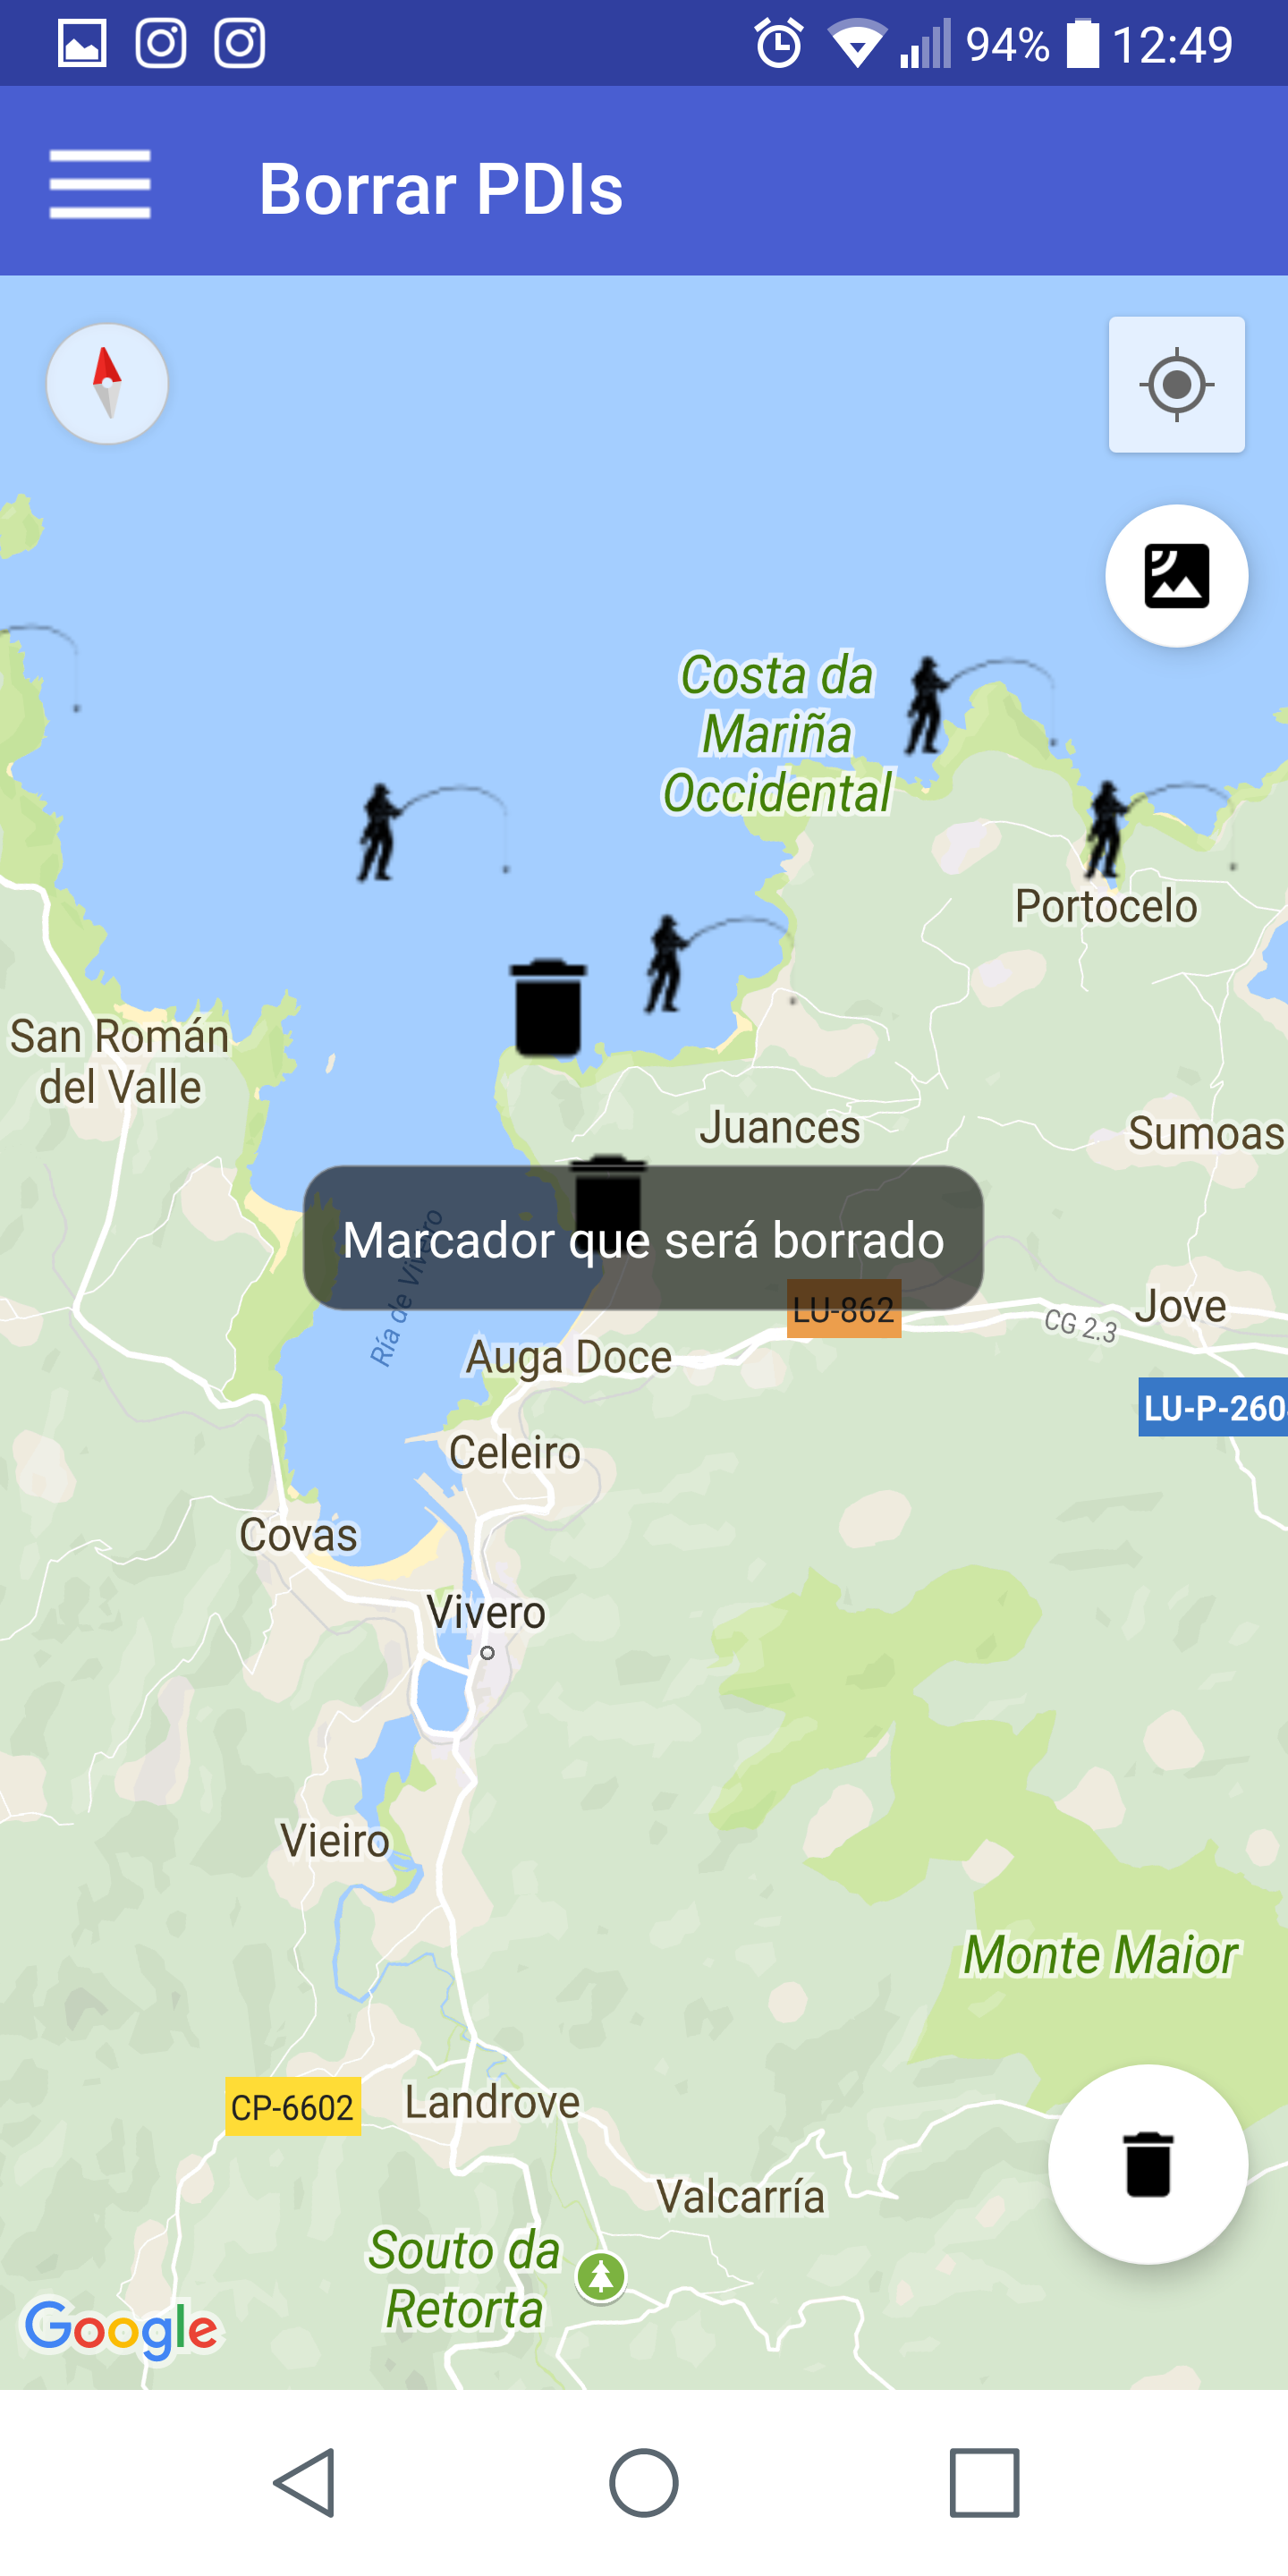
\includegraphics[width=6cm]{capturamovil/pdiborrar.png}
 \label{figura2}
\caption{Borrar PDI }

\end{minipage}
\end{figure}



\subsection{Sprint 4}

En este Sprint nos centraremos en la historia \textbf{\textit{Iniciar sesión }}, que contiene los siguientes casos de uso:



\begin{itemize}
\item\textbf{ \textit{R1  Registrarse en la aplicación.}}
\item \textbf{\textit{R2 Iniciar sesión en la aplicación. }}

\end{itemize} 
\begin{figure}[htbp]
\begin{minipage}[b]{0.5\linewidth} %Una minipágina que cubre la mitad de la página
\centering
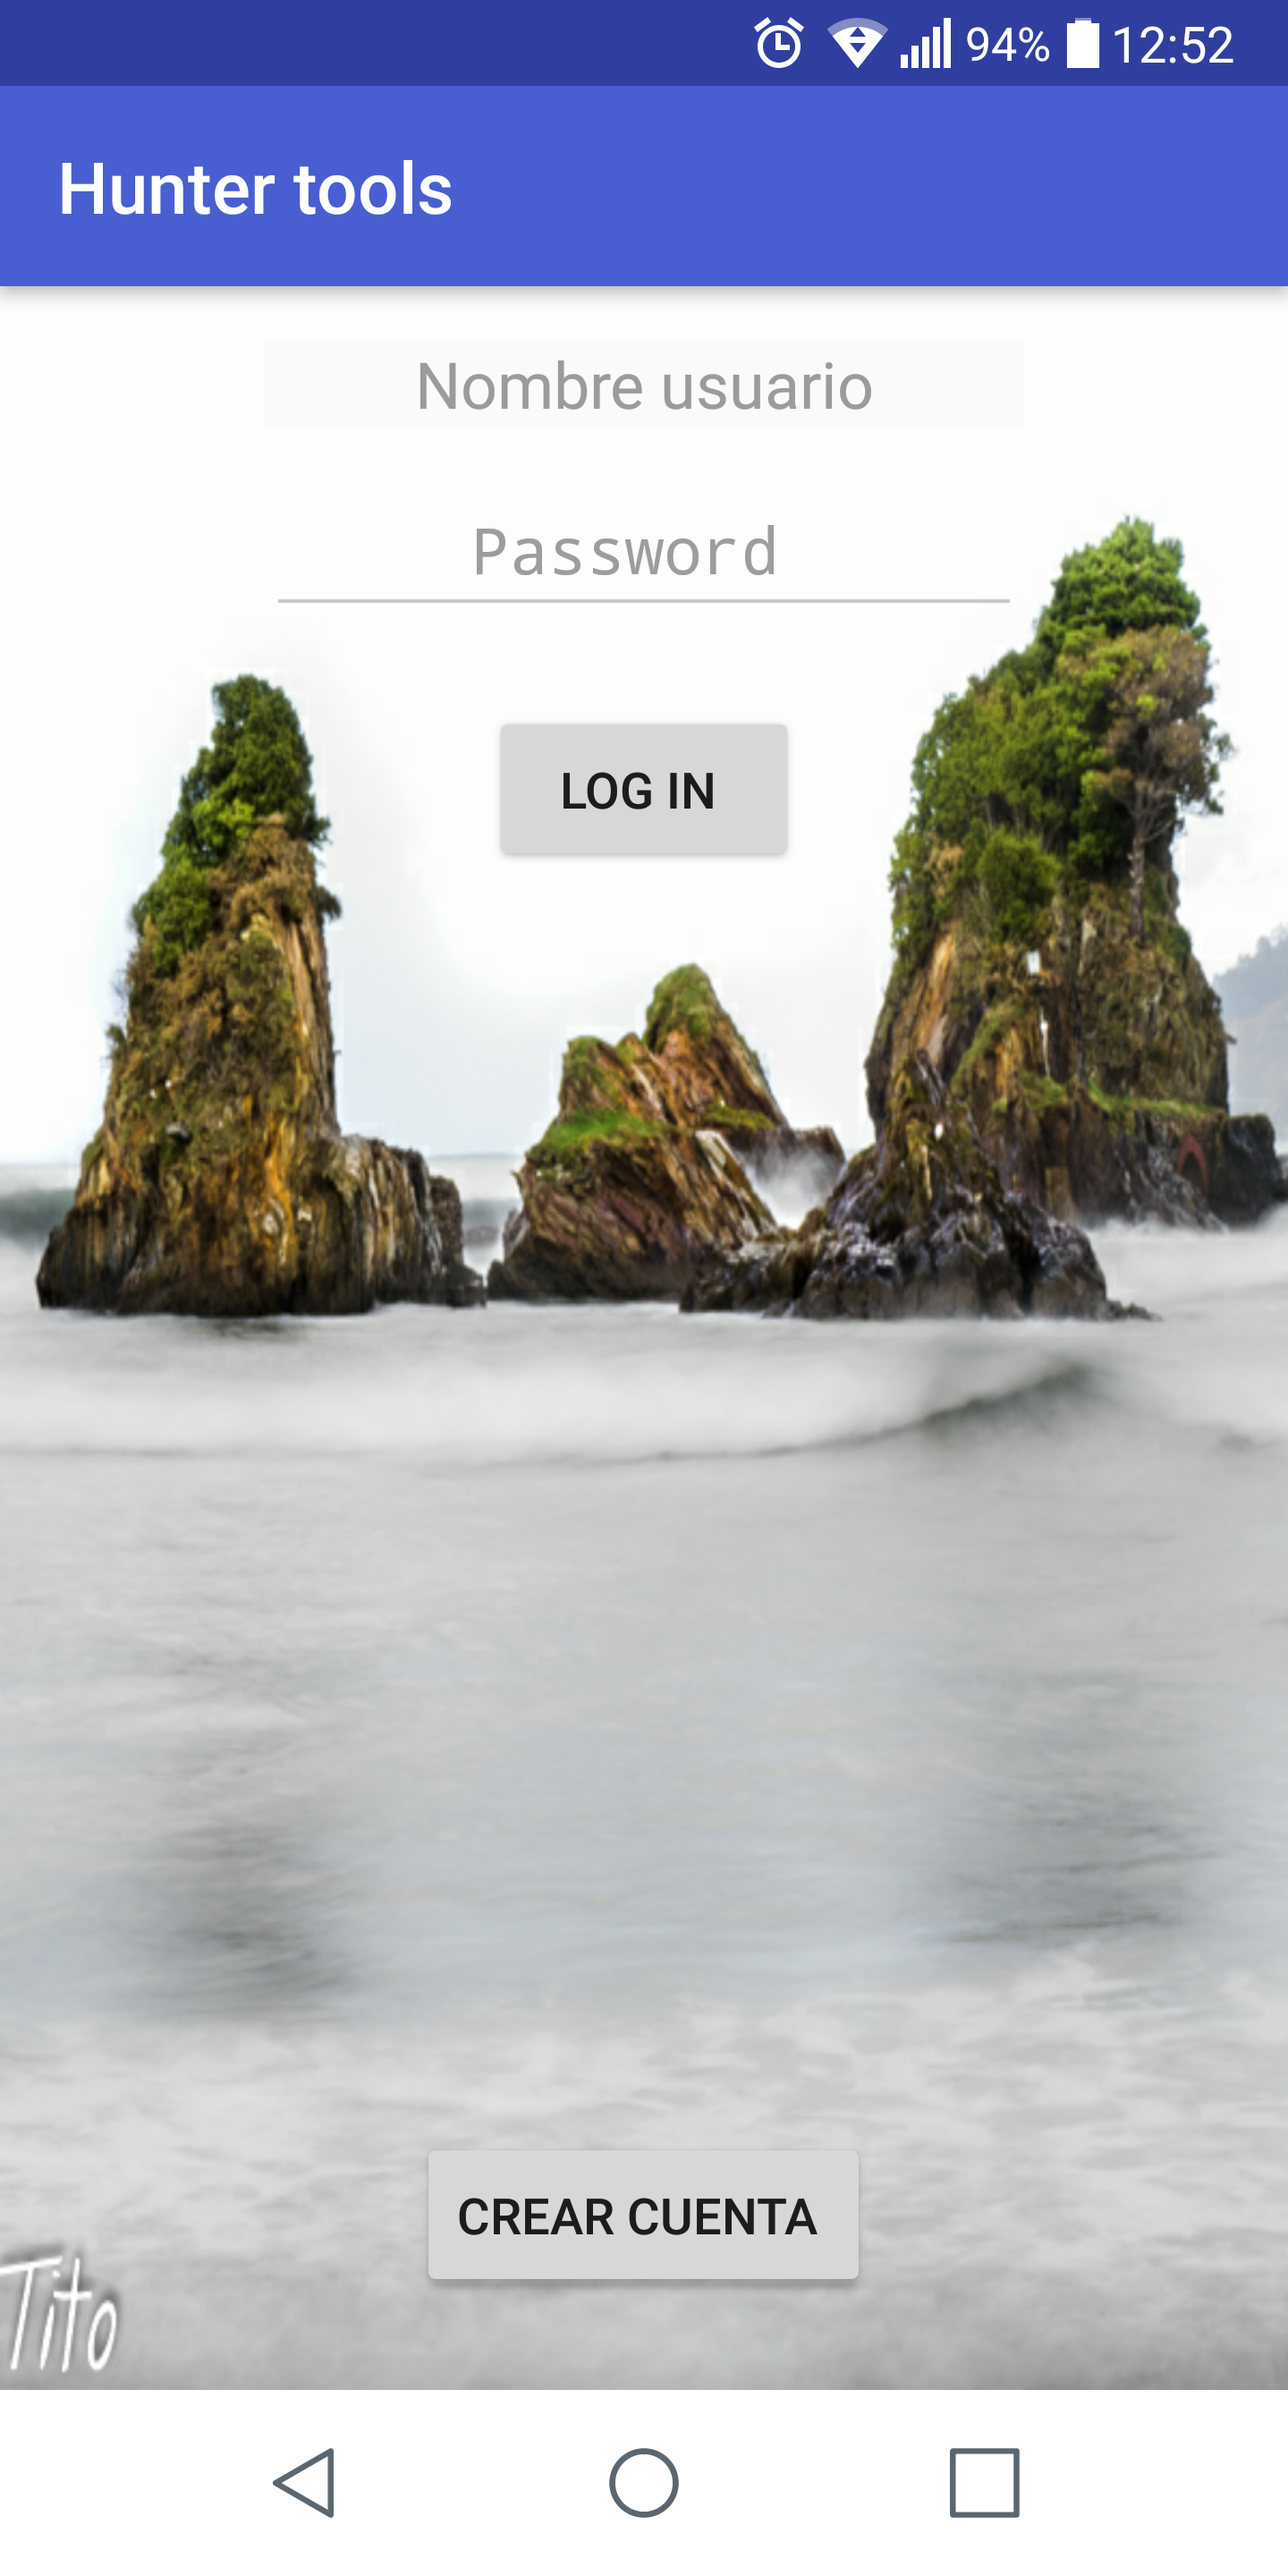
\includegraphics[width=6cm]{capturamovil/login.png}
 \label{figura1}
\caption{Iniciar sesión }

\end{minipage}
\hspace{0.5cm} % Si queremos tener un poco de espacio entre las dos figuras
\begin{minipage}[b]{0.5\linewidth}
\centering
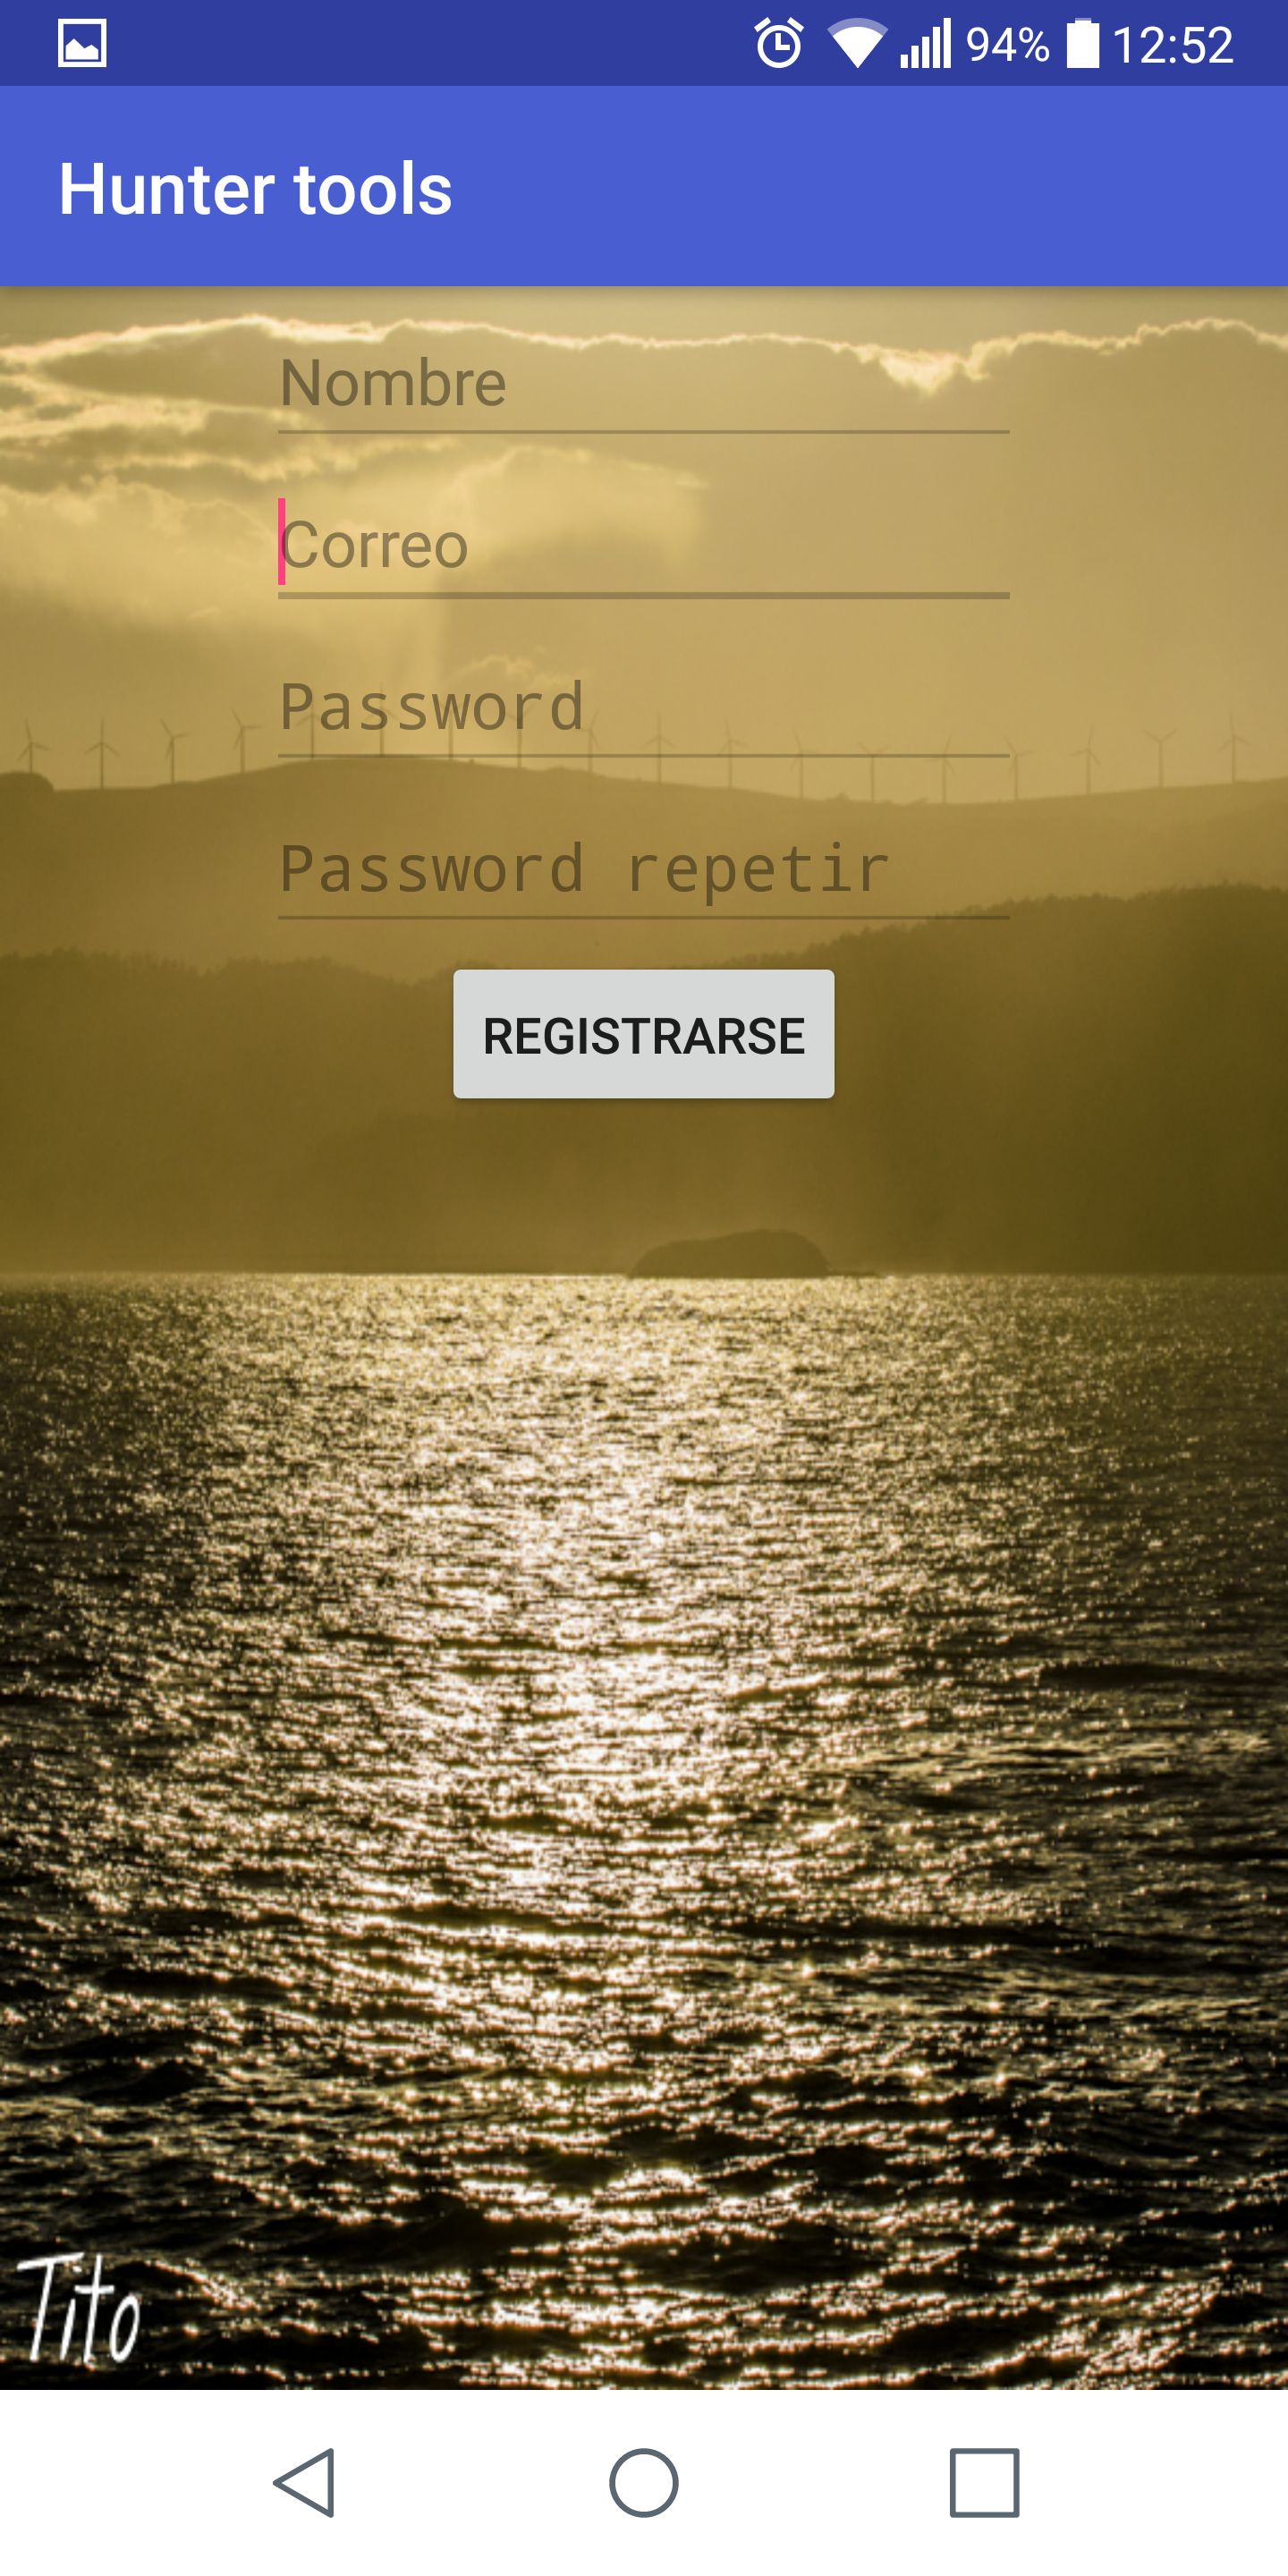
\includegraphics[width=6cm]{capturamovil/registro.png}
 \label{figura2}
\caption{Registro del usuario }

\end{minipage}
\end{figure}
Además en este Sprint hemos desarrollado un toolbar para gestionar todas las opciones y mejorar la navegación del usuario en la aplicación.
\begin{figure}[H]
		\centering
		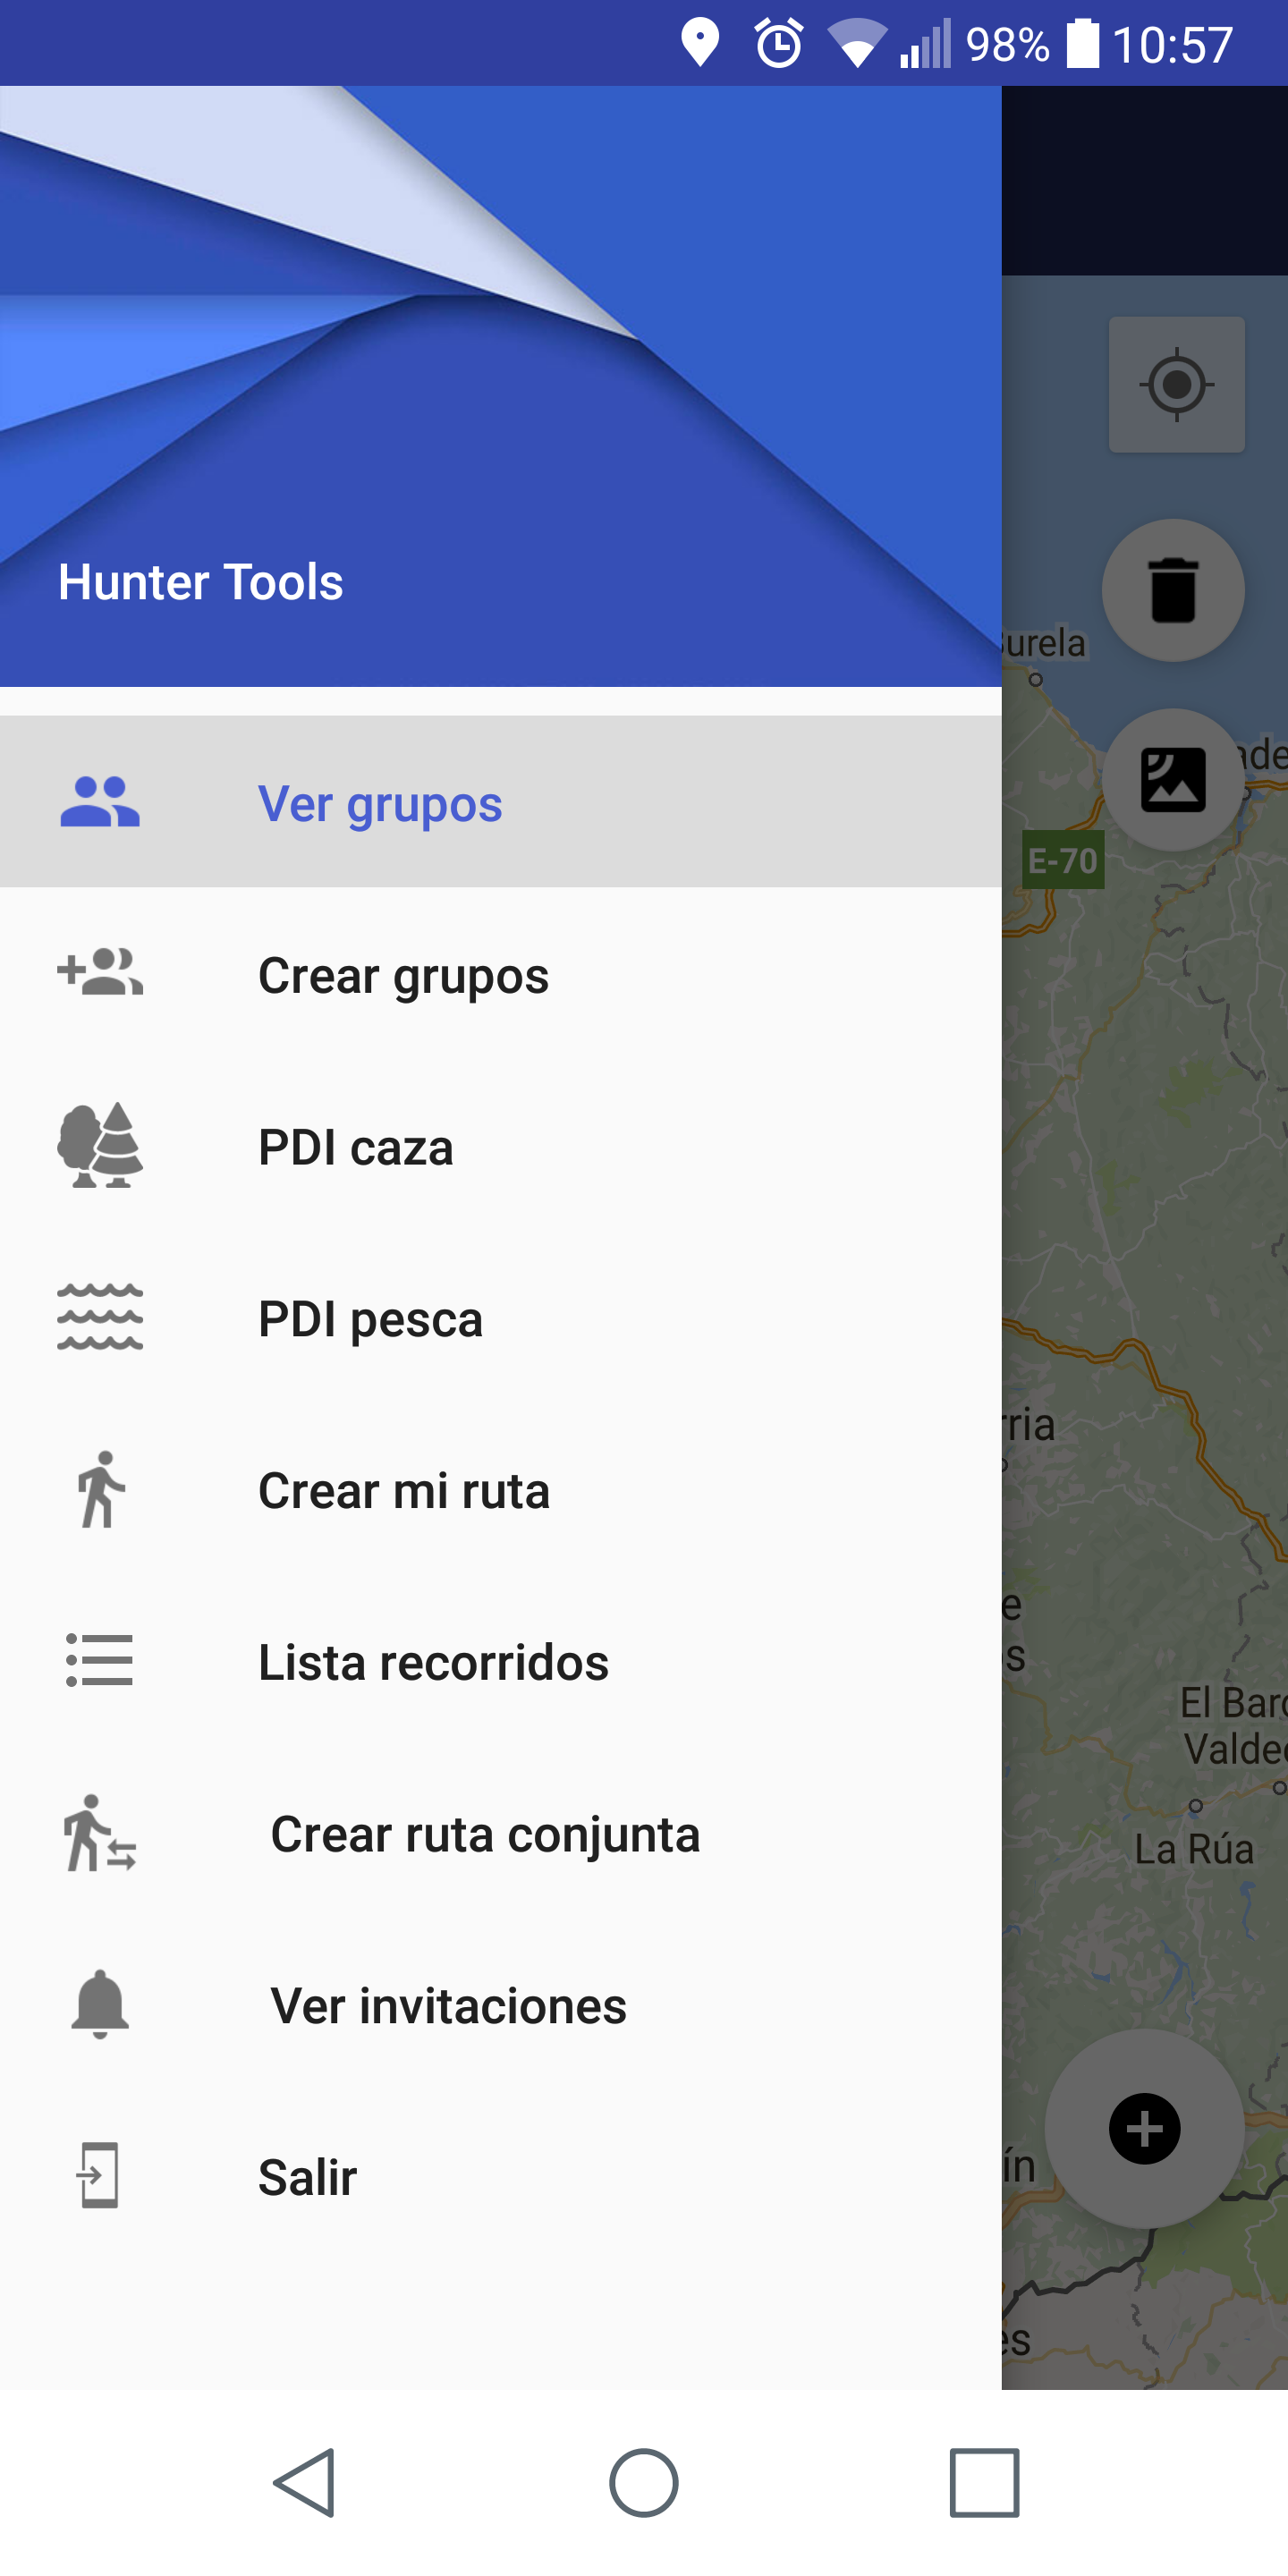
\includegraphics[width=0.3\textwidth] {capturamovil/opciones}
		\caption{Captura del menú de navegación}
	\end{figure}
\subsection{Sprint 5}
Este Sprint se centrará en la historia \textbf{\textit{Gestión de grupos}} que contiene los siguientes casos de uso:
\begin{itemize}
\item\textbf{ \textit{R-G-1 Crear grupo}}
\item\textbf{\textit{ R-G-2 Añadir integrantes}}
\item \textbf{\textit{R-G-3 Eliminar integrantes}},
\item \textbf{\textit{R-G-4 Ver grupos}}.
\item \textbf{\textit{R-G-5 Ver integrantes grupo}}
\end{itemize}
\begin{figure}[htbp]
\begin{minipage}[b]{0.5\linewidth} %Una minipágina que cubre la mitad de la página
\centering
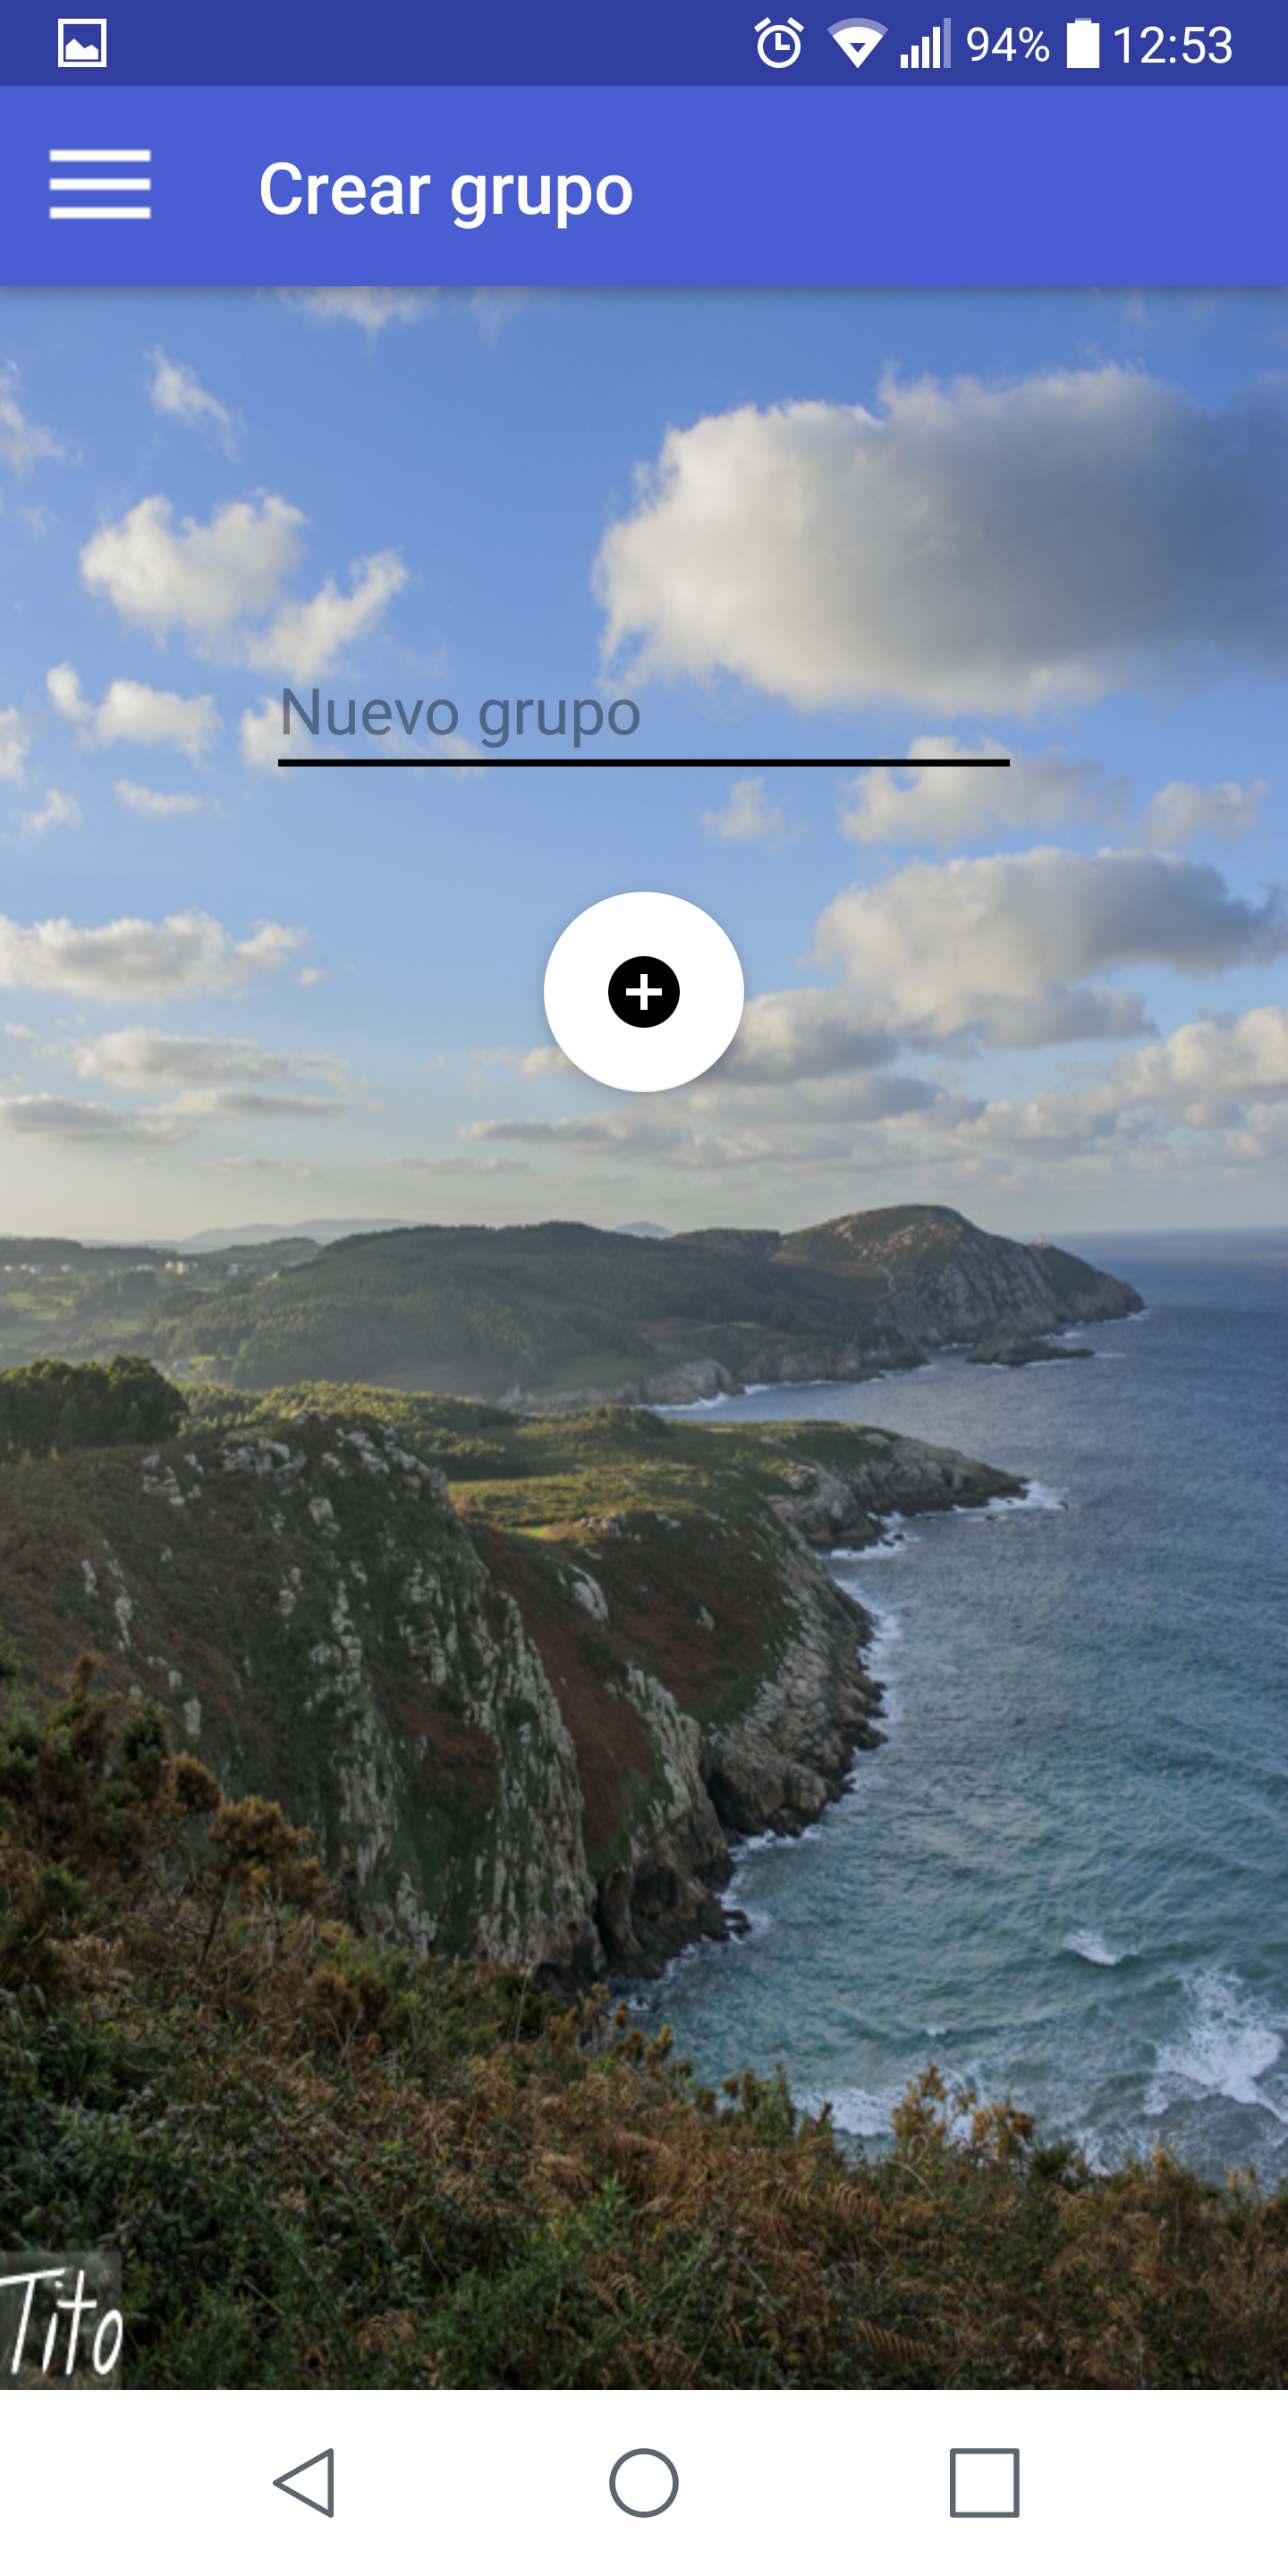
\includegraphics[width=6cm]{capturamovil/creargrupo.png}
 \label{figura1}
\caption{Crear grupo}

\end{minipage}
\hspace{0.5cm} % Si queremos tener un poco de espacio entre las dos figuras
\begin{minipage}[b]{0.5\linewidth}
\centering
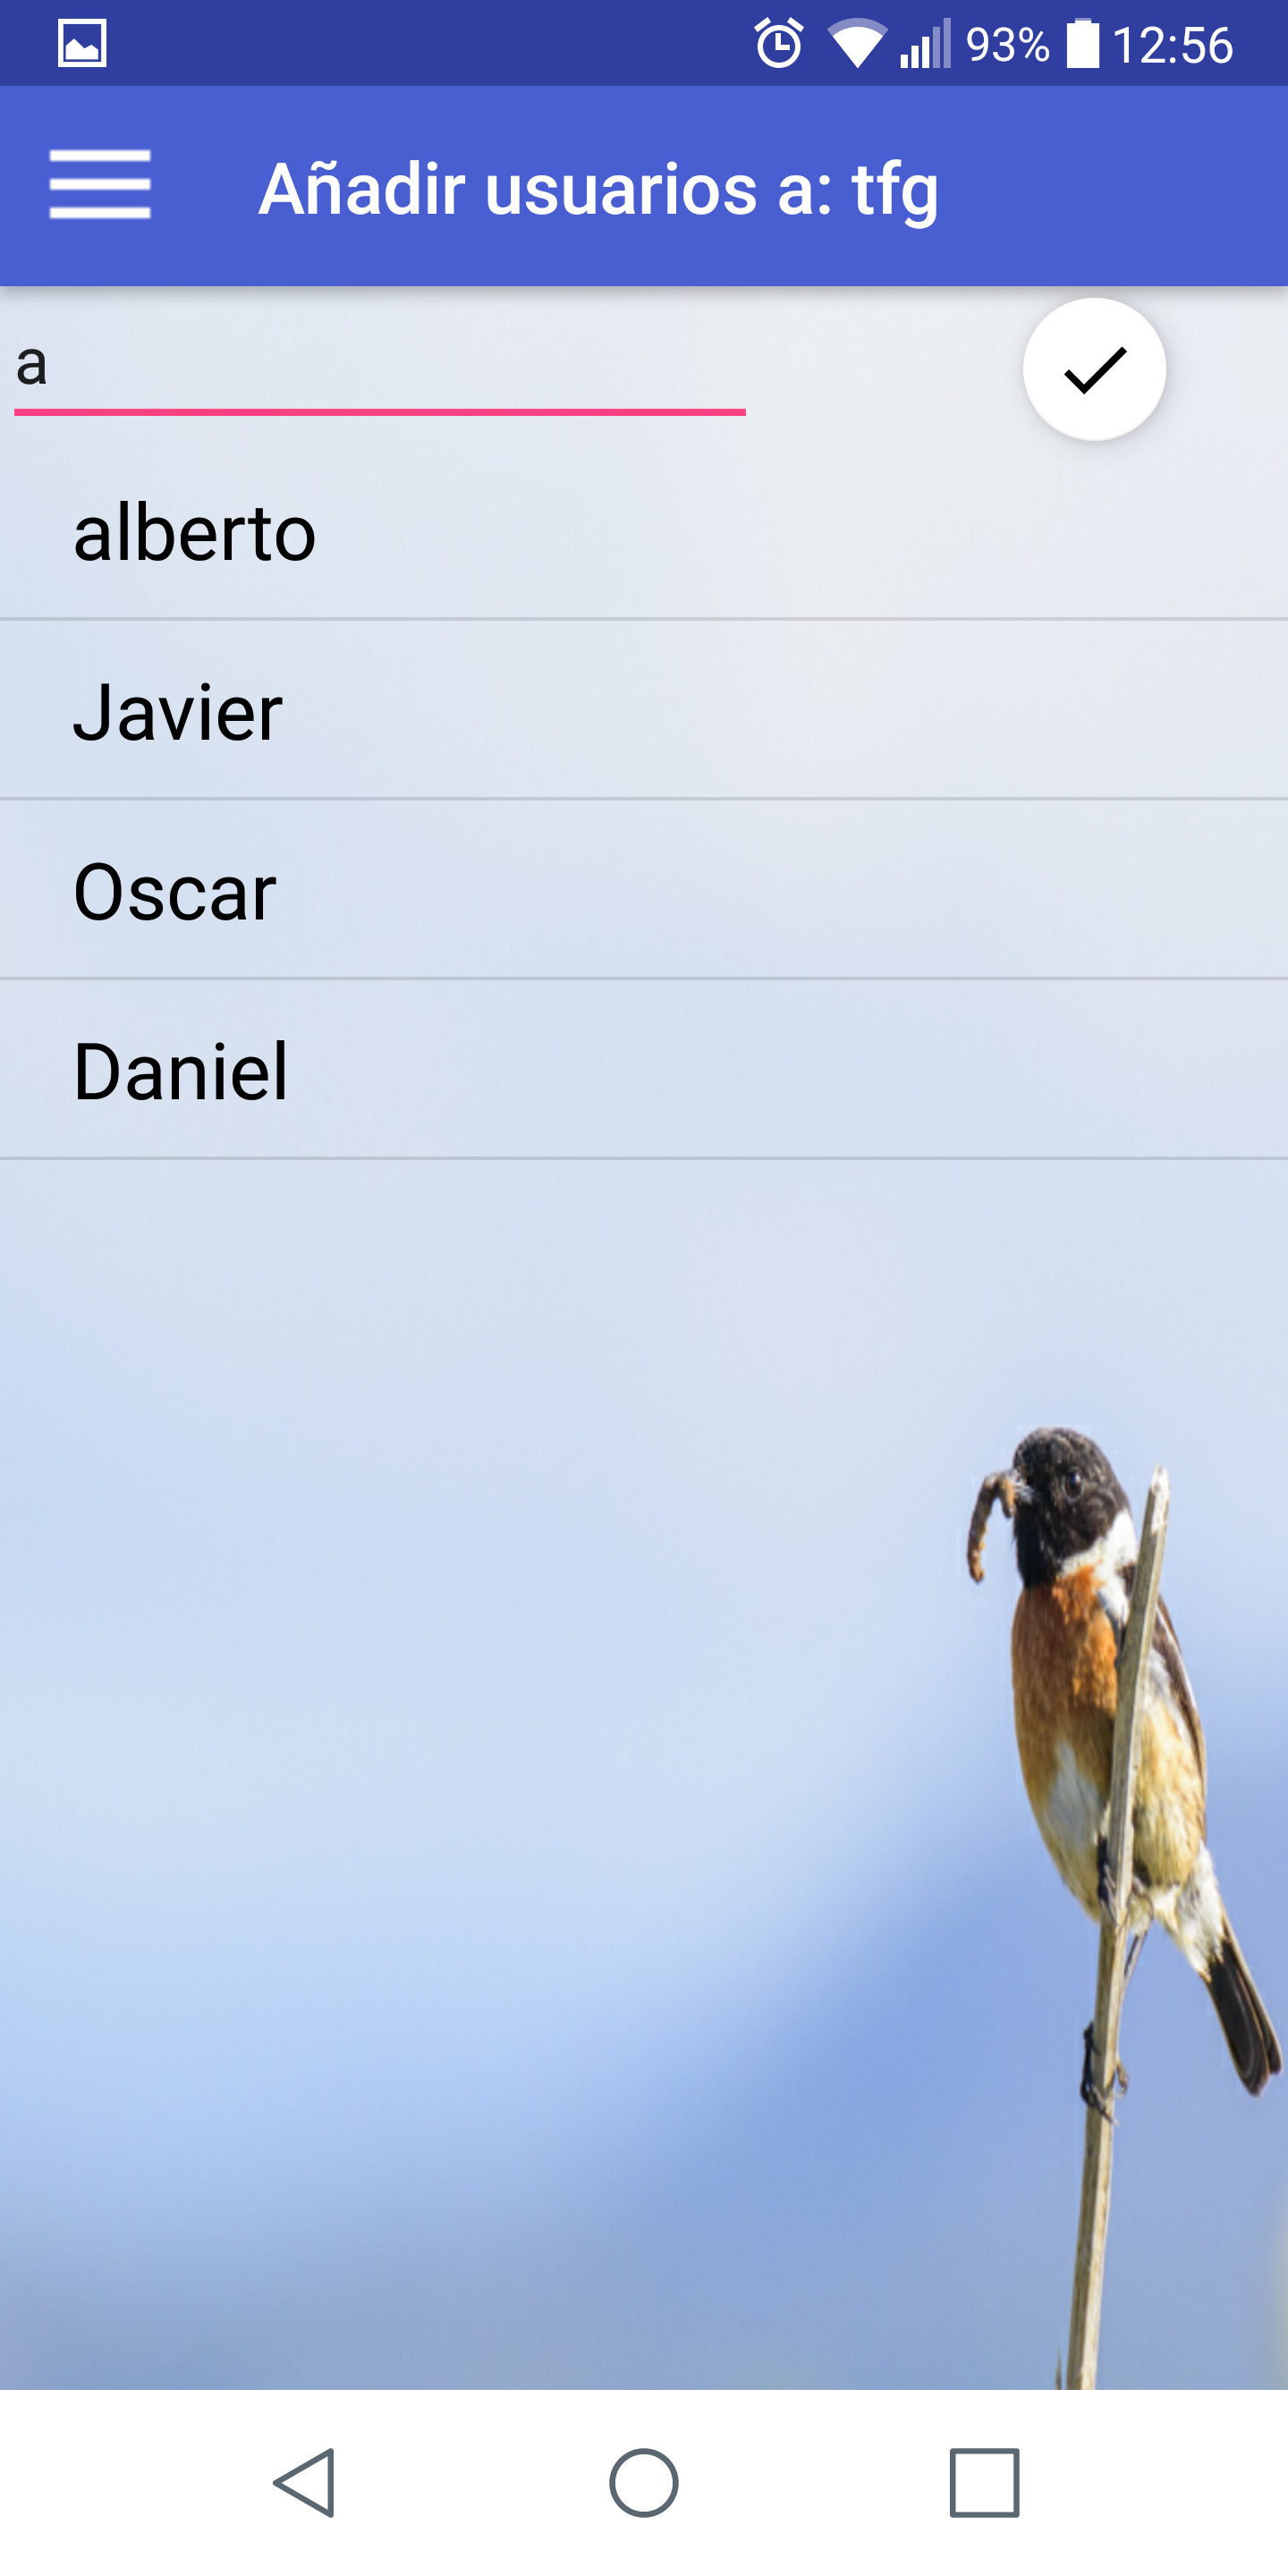
\includegraphics[width=6cm]{capturamovil/addintegrante.png}
 \label{figura2}
\caption{Añadir usuarios a grupo }

\end{minipage}
\end{figure}


\begin{figure}[htbp]
\begin{minipage}[b]{0.5\linewidth} %Una minipágina que cubre la mitad de la página
\centering
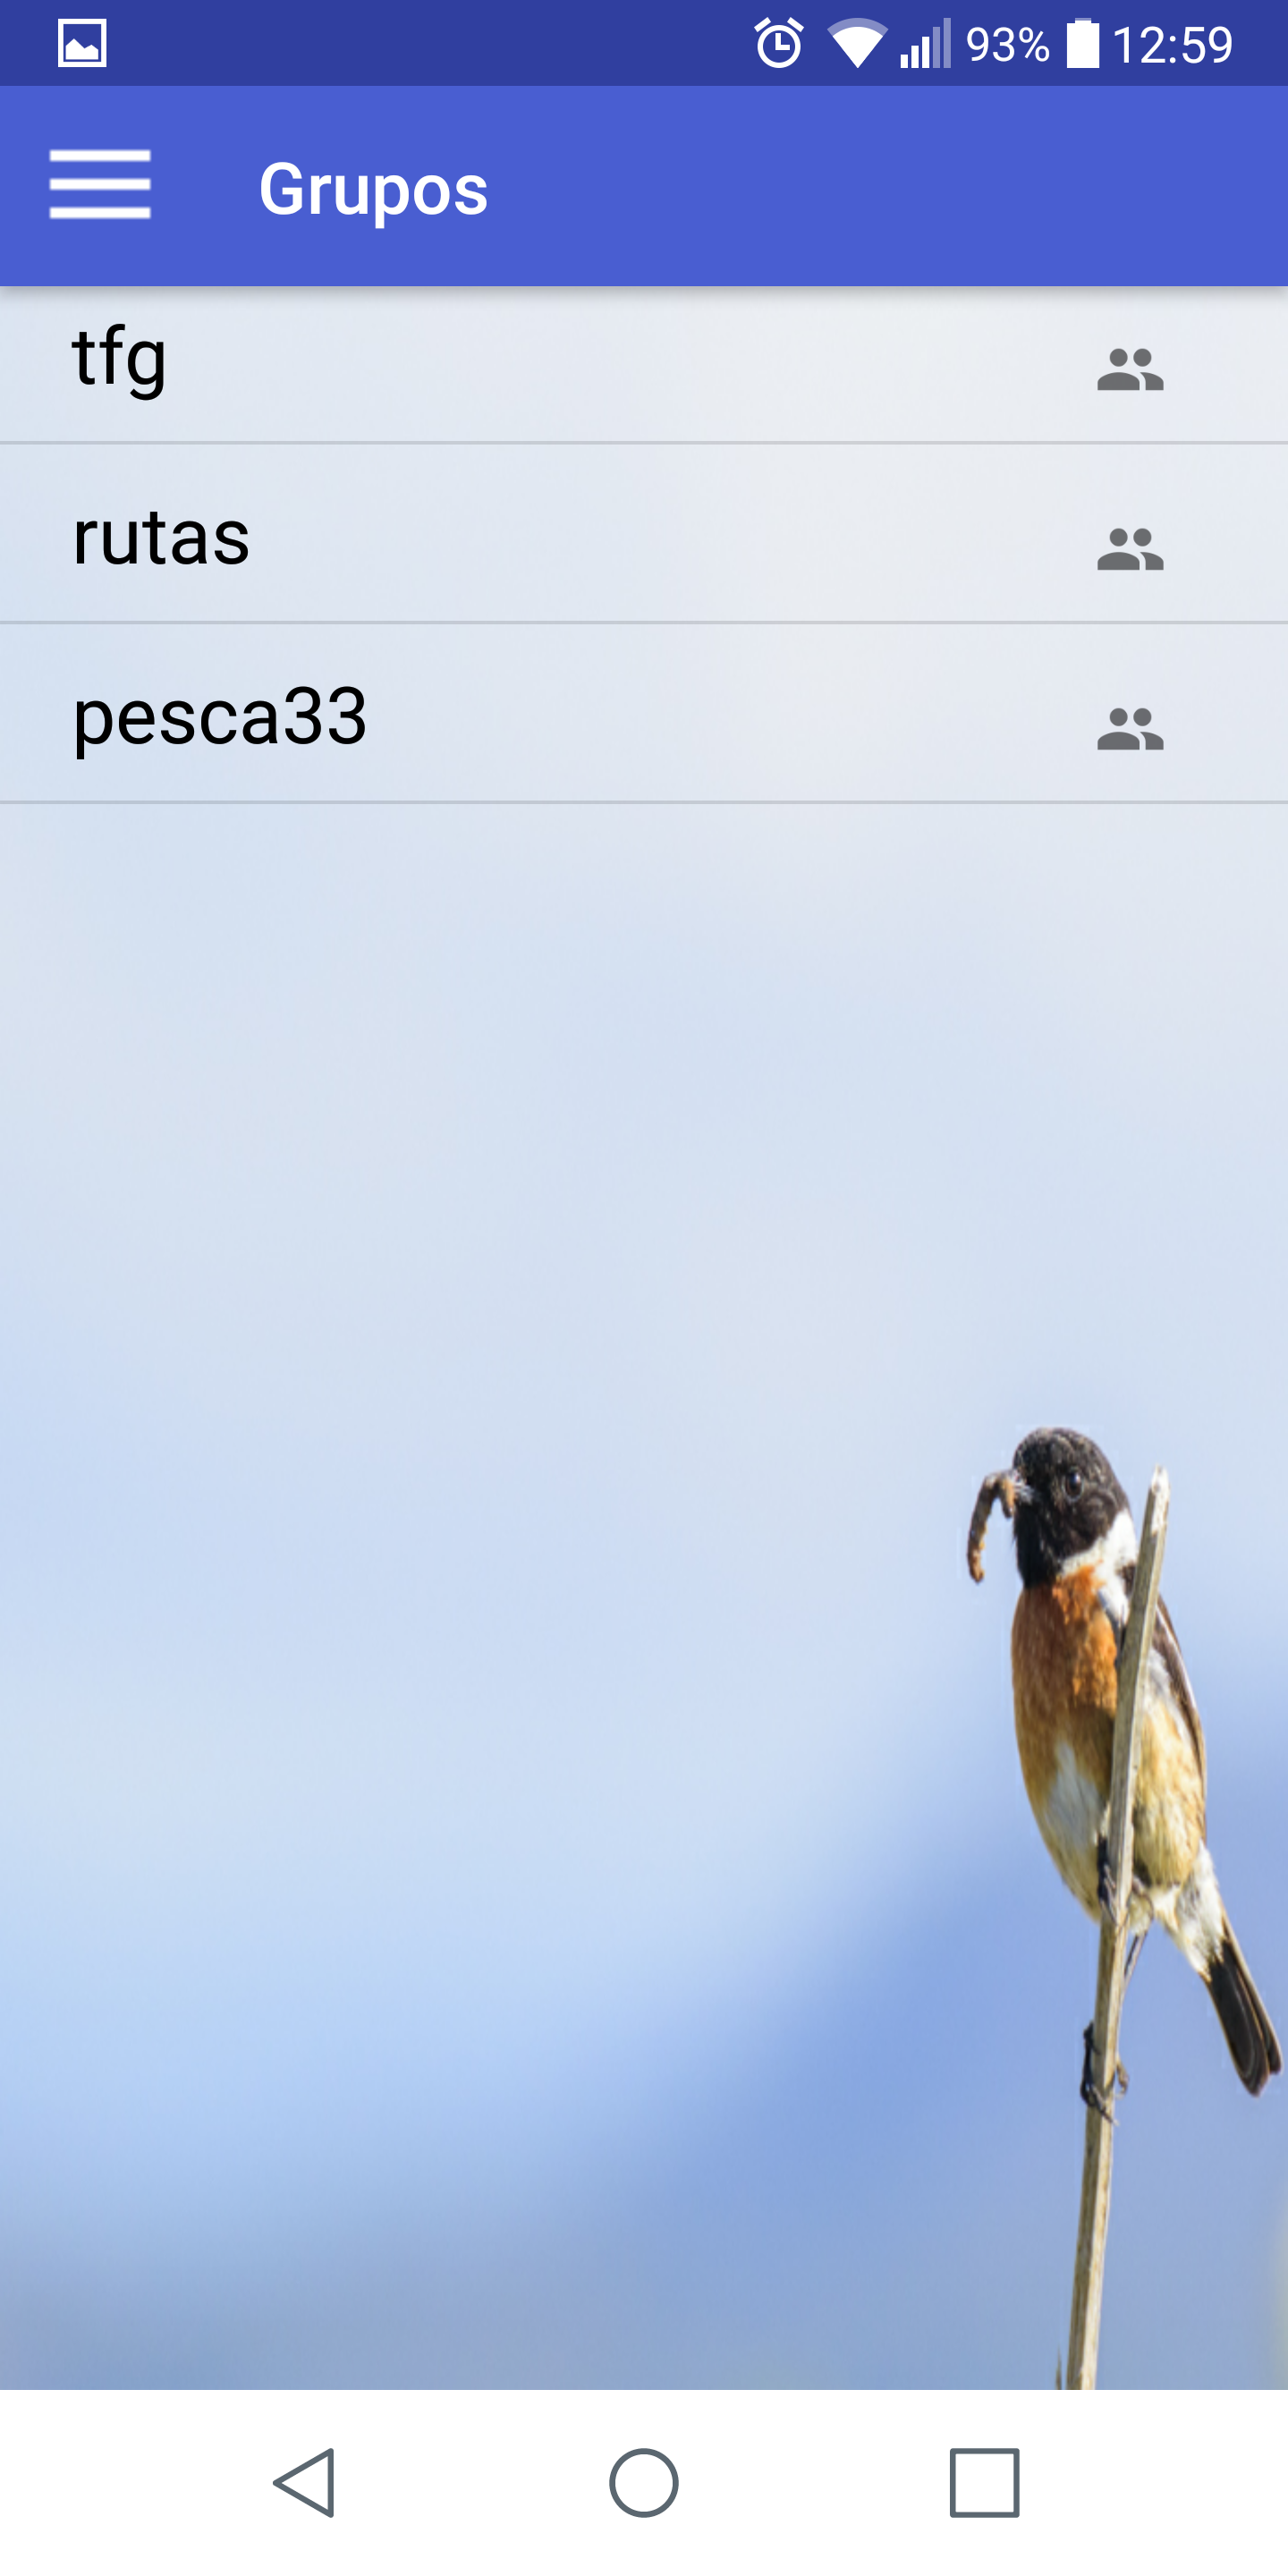
\includegraphics[width=6cm]{capturamovil/vergrupos.png}
 \label{figura1}
\caption{Ver grupos del usuario}

\end{minipage}
\hspace{0.5cm} % Si queremos tener un poco de espacio entre las dos figuras
\begin{minipage}[b]{0.5\linewidth}
\centering
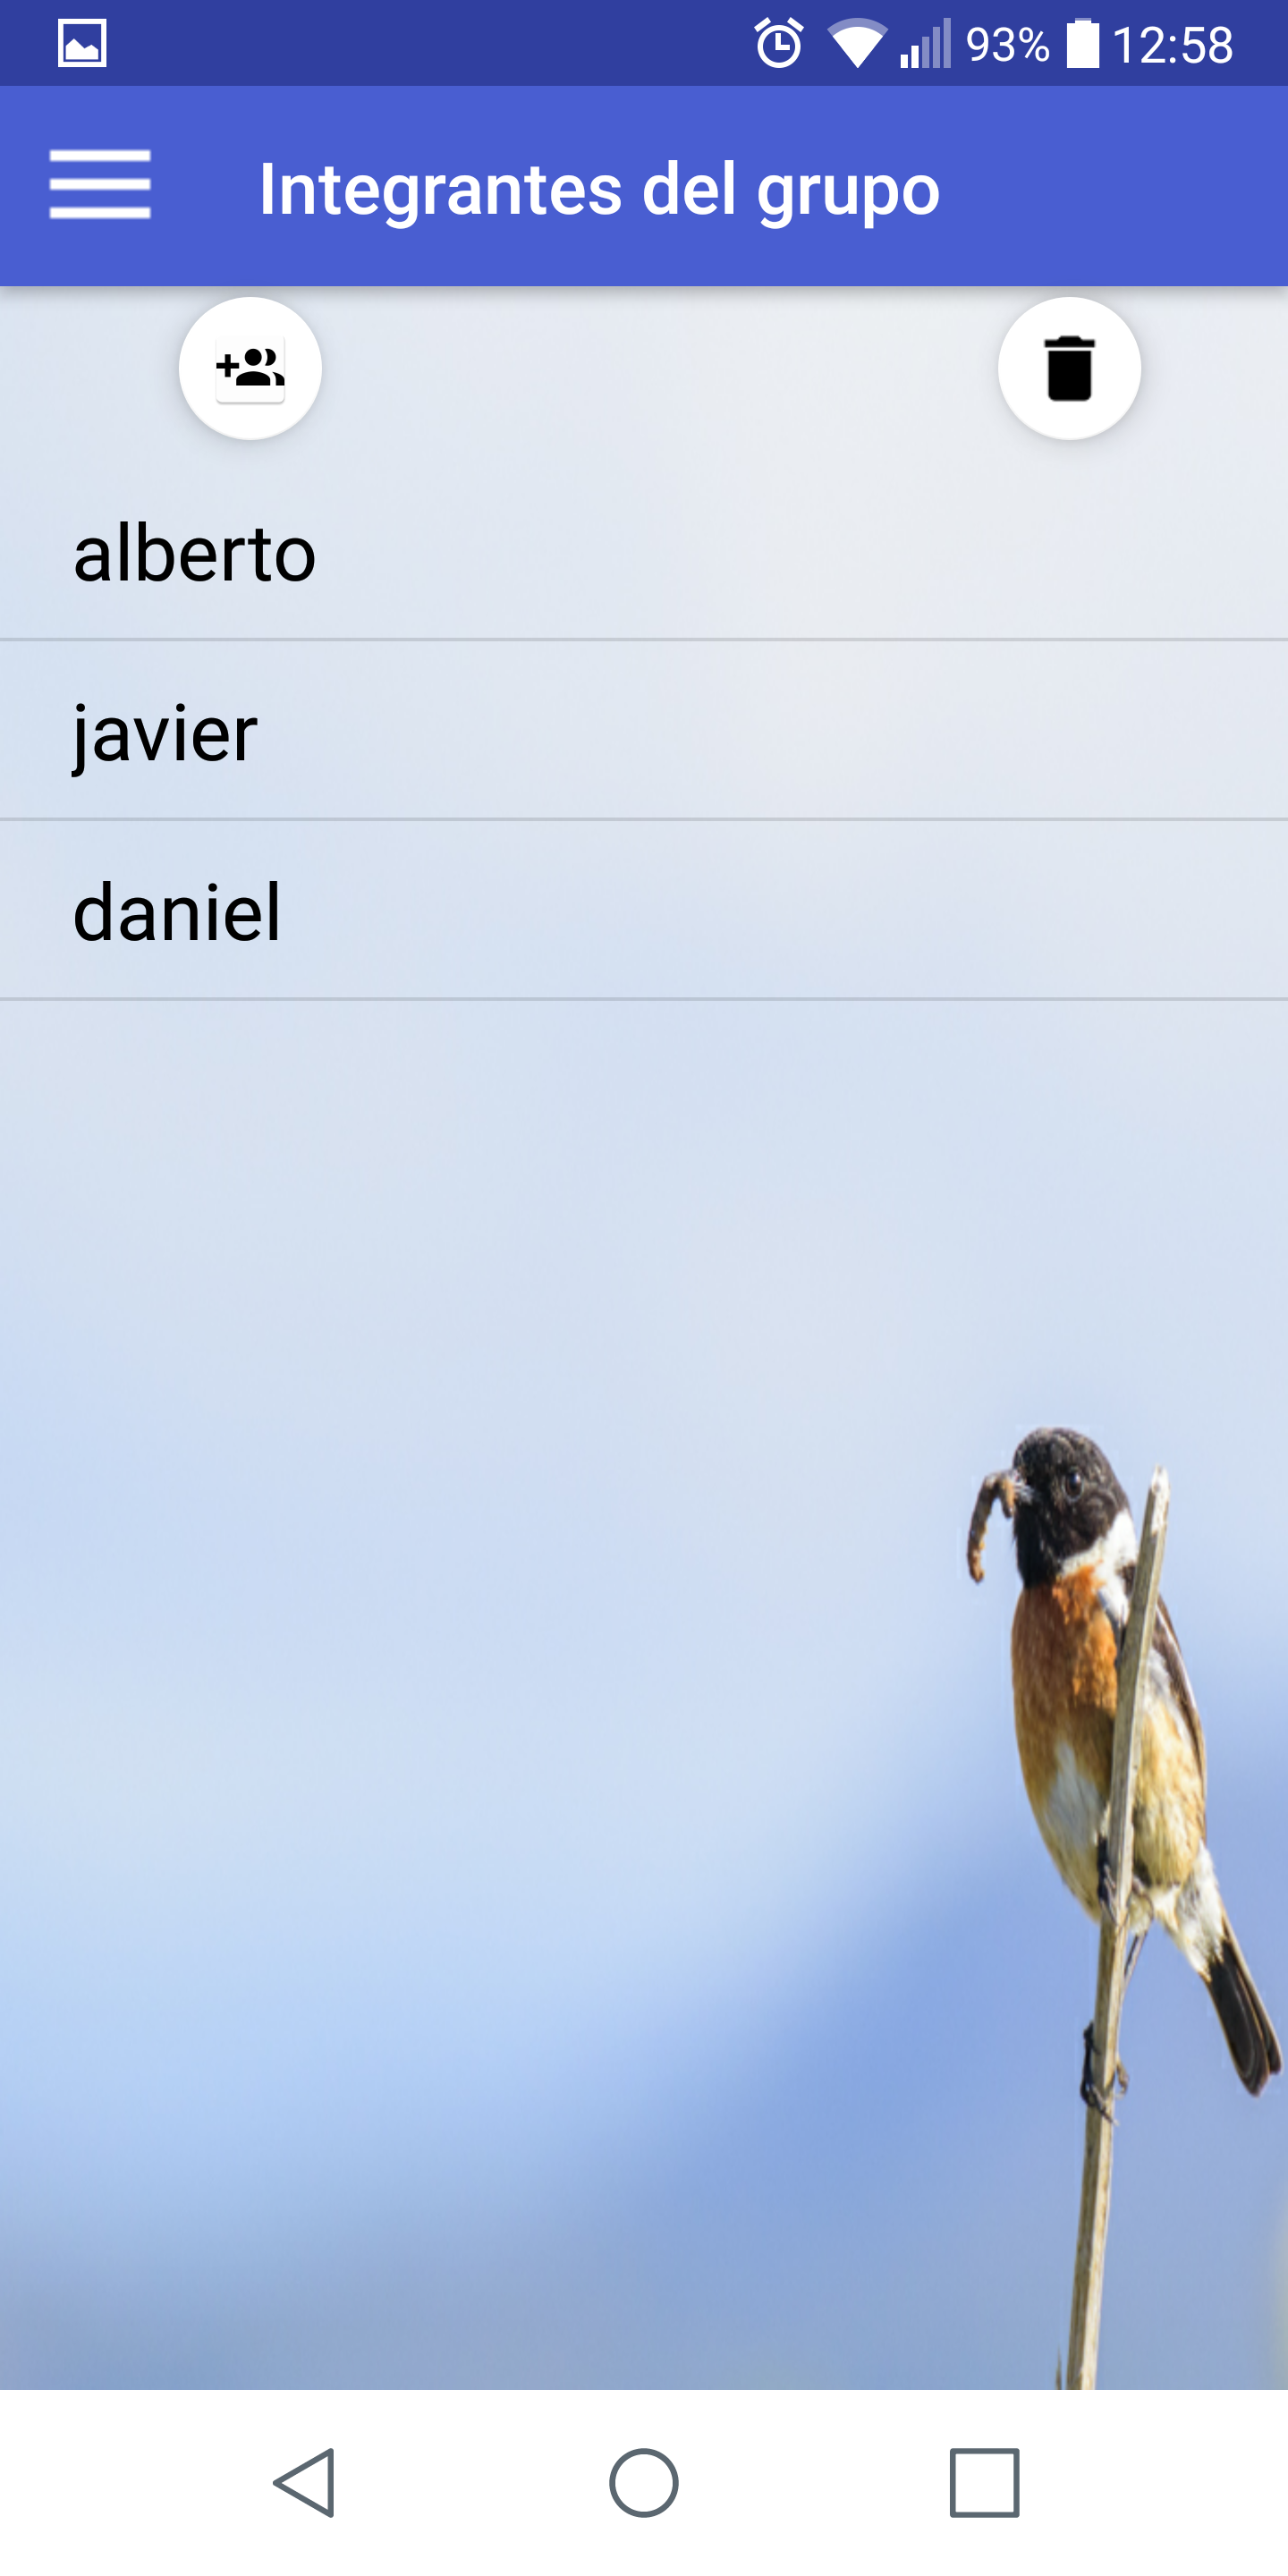
\includegraphics[width=6cm]{capturamovil/verintegrantes.png}
 \label{figura2}
\caption{Ver integrantes del grupo }

\end{minipage}
\end{figure}
\newpage
\subsection{Sprint 6}
Este Sprint se centrará en \textbf{\textit{Iniciar una ruta individual}}.

\begin{itemize}
\item \textbf{\textit{R-R-1 Crear ruta}}
\item \textbf{\textit{R-R-1.1 Iniciar ruta}}
\item\textbf{ \textit{R-R-1.2 Parar ruta}}
\item \textbf{\textit{R-R-1.3 Guardar ruta}}
\item \textbf{\textit{R-R-3 Listar rutas} }
\item \textbf{\textit{R-R-4 Ver ruta en mapa}}
\item \textbf{\textit{R-R-5 Eliminar ruta}}
\end{itemize}

\begin{figure}[htbp]
\begin{minipage}[b]{0.5\linewidth} %Una minipágina que cubre la mitad de la página
\centering
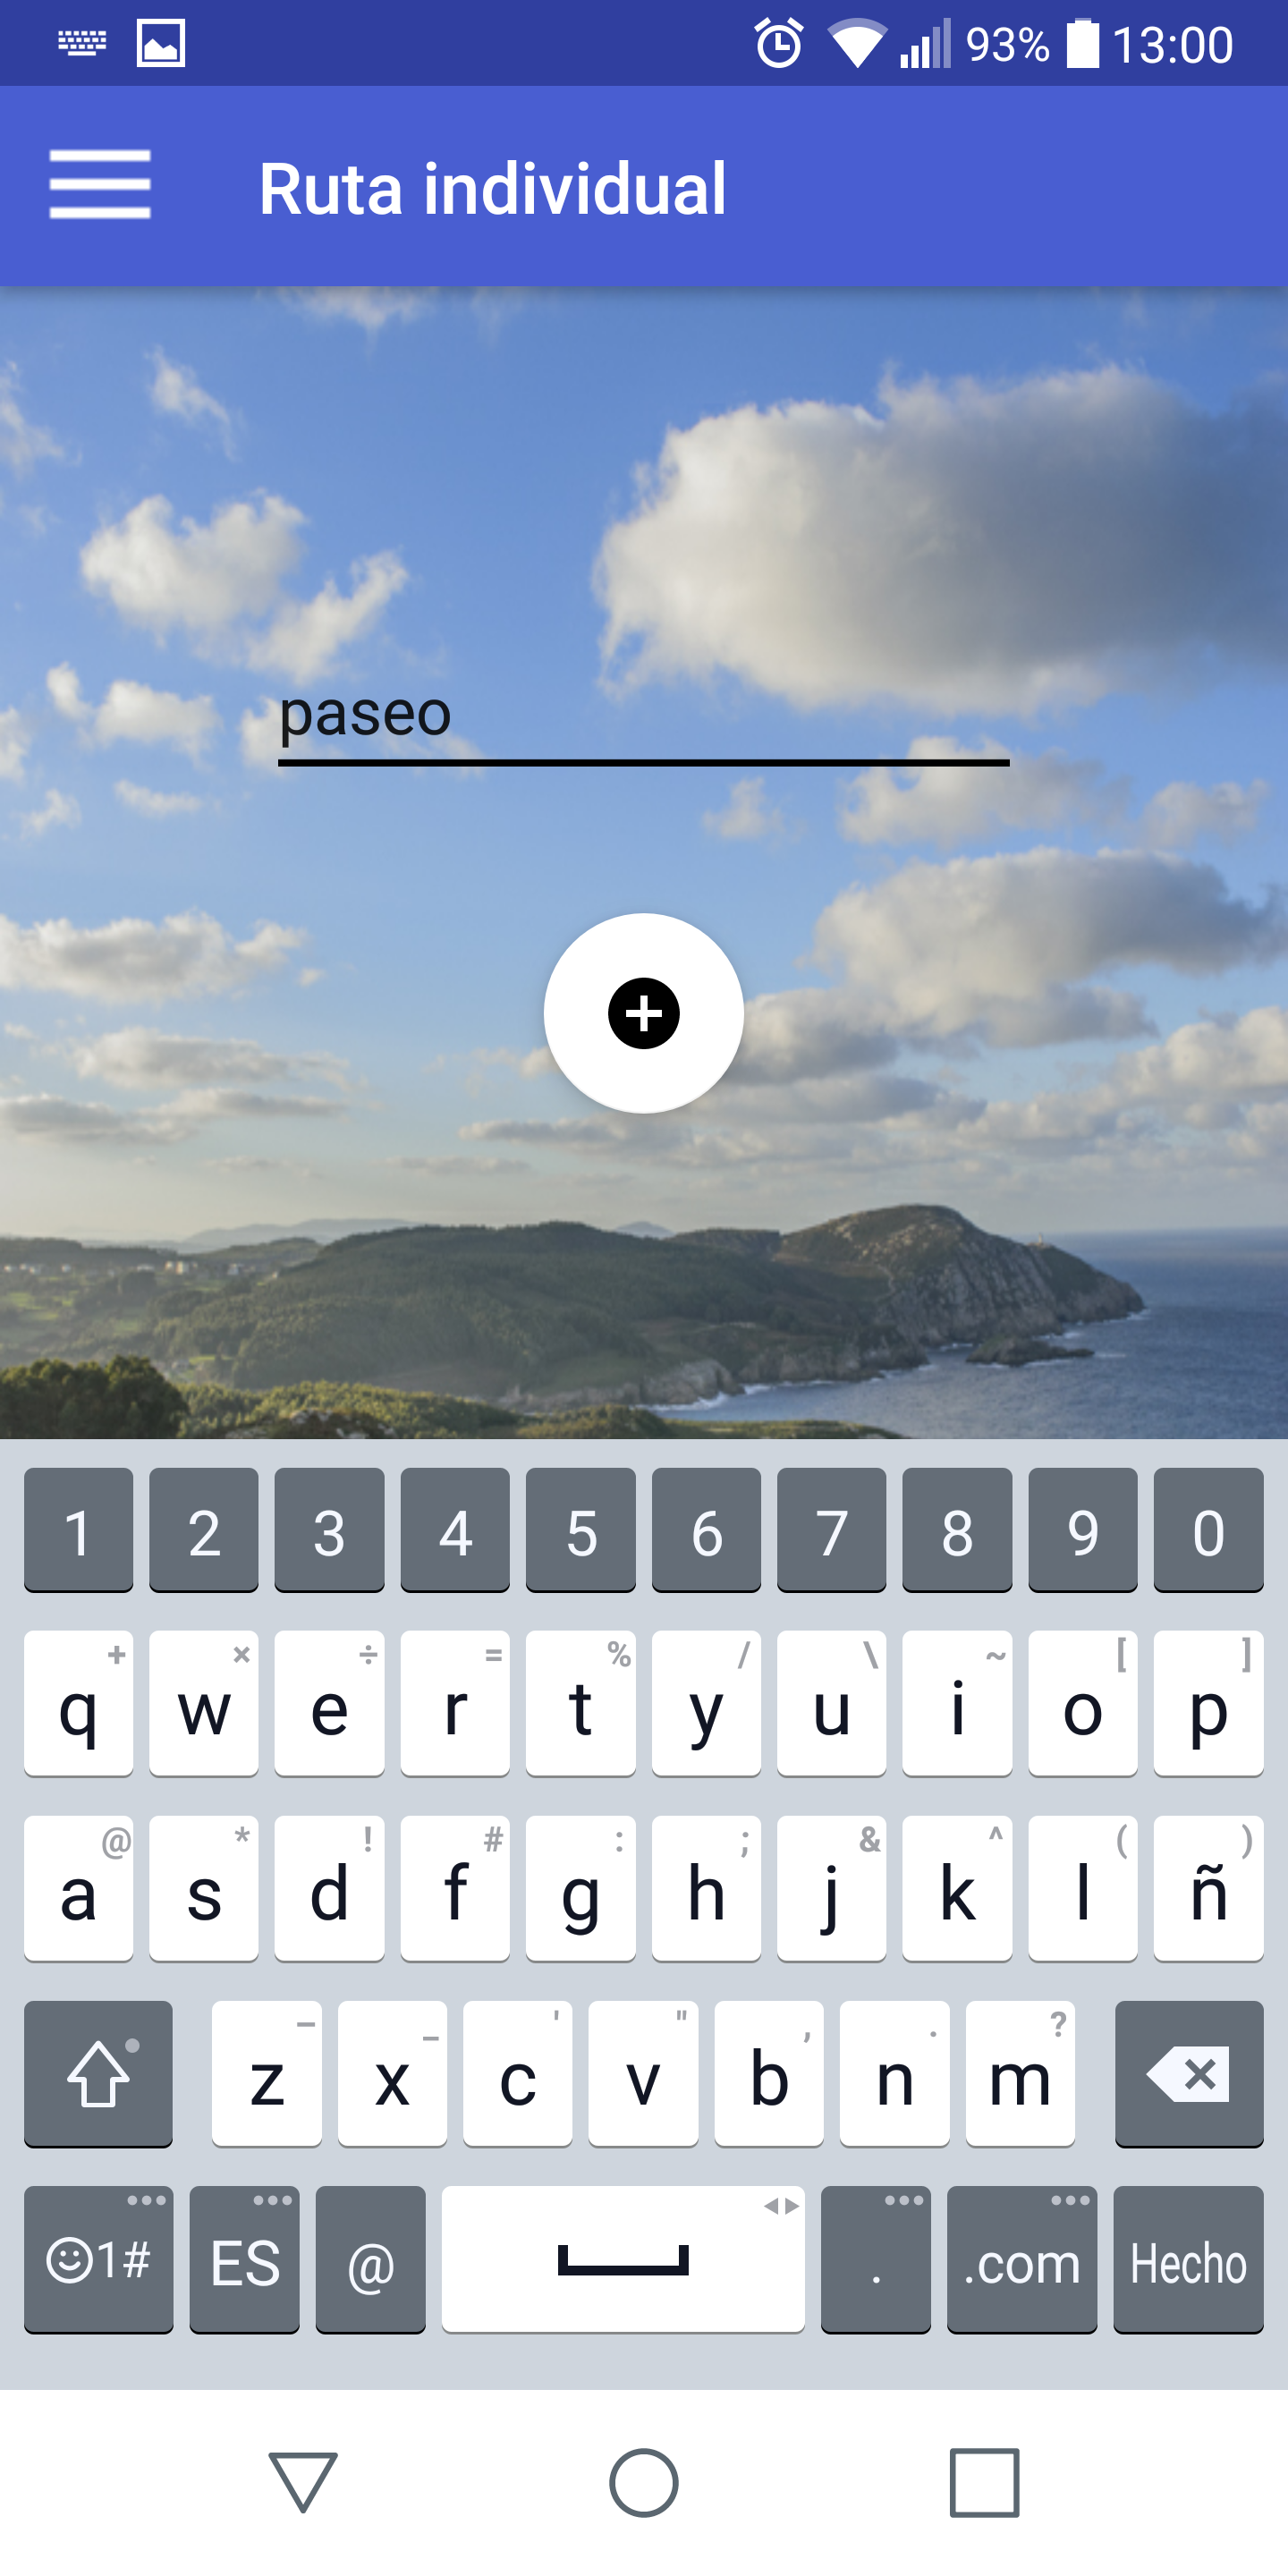
\includegraphics[width=6cm]{capturamovil/crearruta.png}
 \label{figura1}
\caption{Crear ruta}

\end{minipage}
\hspace{0.5cm} % Si queremos tener un poco de espacio entre las dos figuras
\begin{minipage}[b]{0.5\linewidth}
\centering
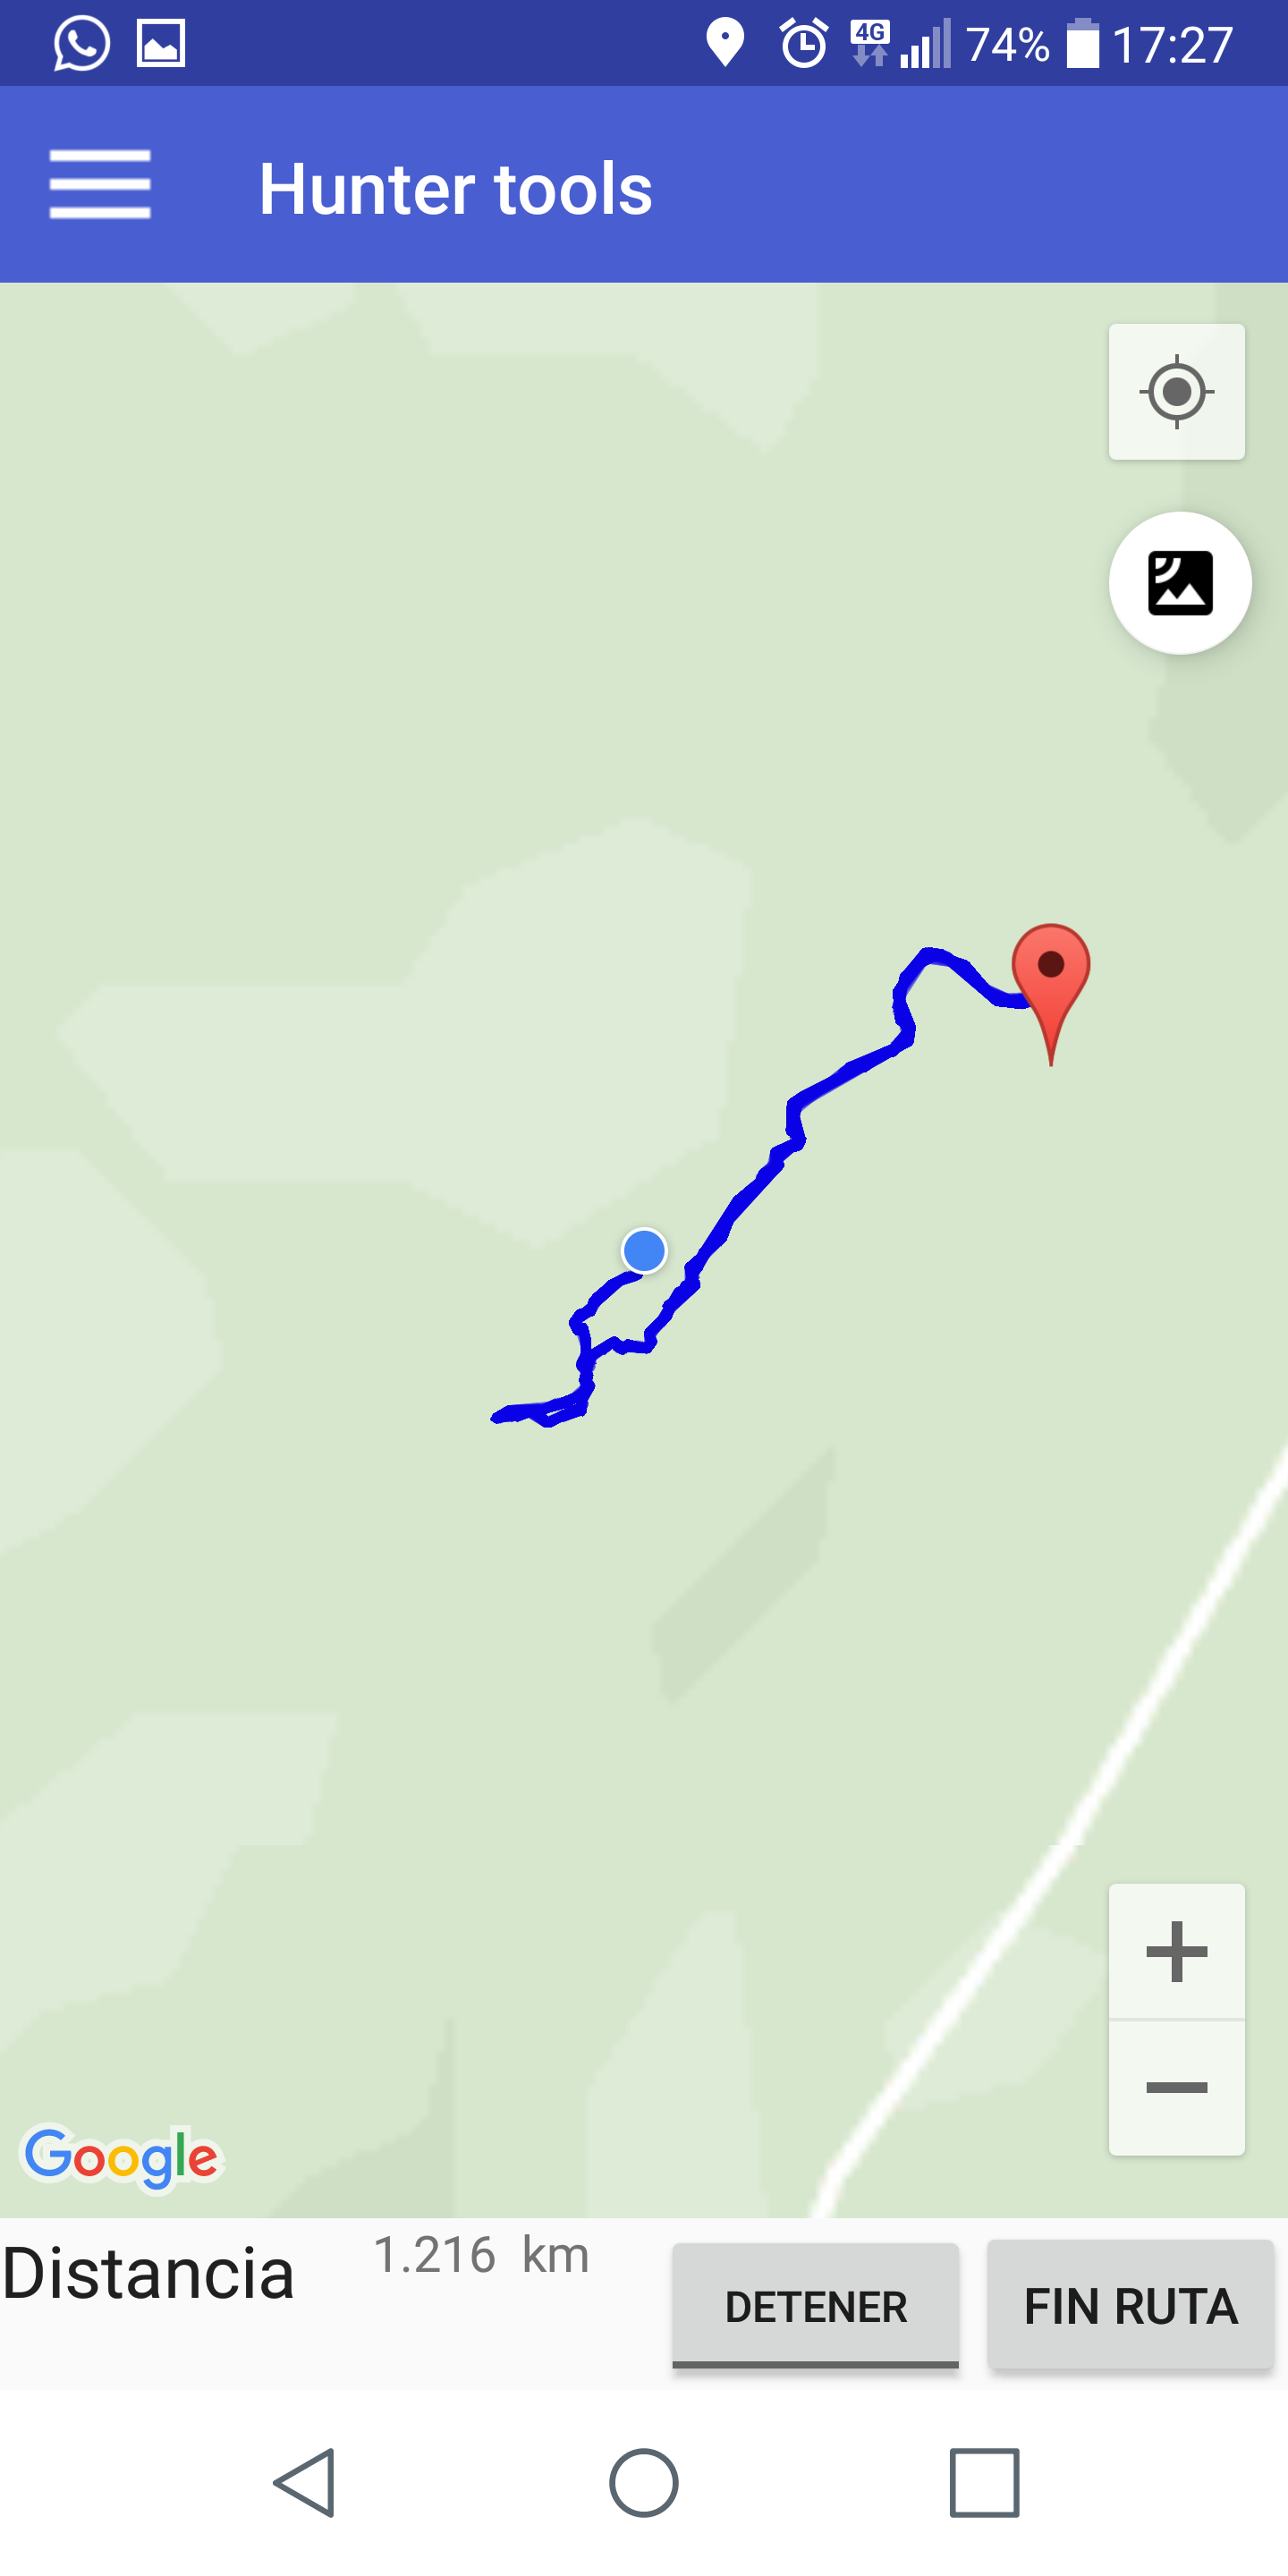
\includegraphics[width=6cm]{capturamovil/individual-navegacion.png}
 \label{figura2}
\caption{Navegación ruta individual }

\end{minipage}
\end{figure}


\begin{figure}[htbp]
\begin{minipage}[b]{0.5\linewidth} %Una minipágina que cubre la mitad de la página
\centering
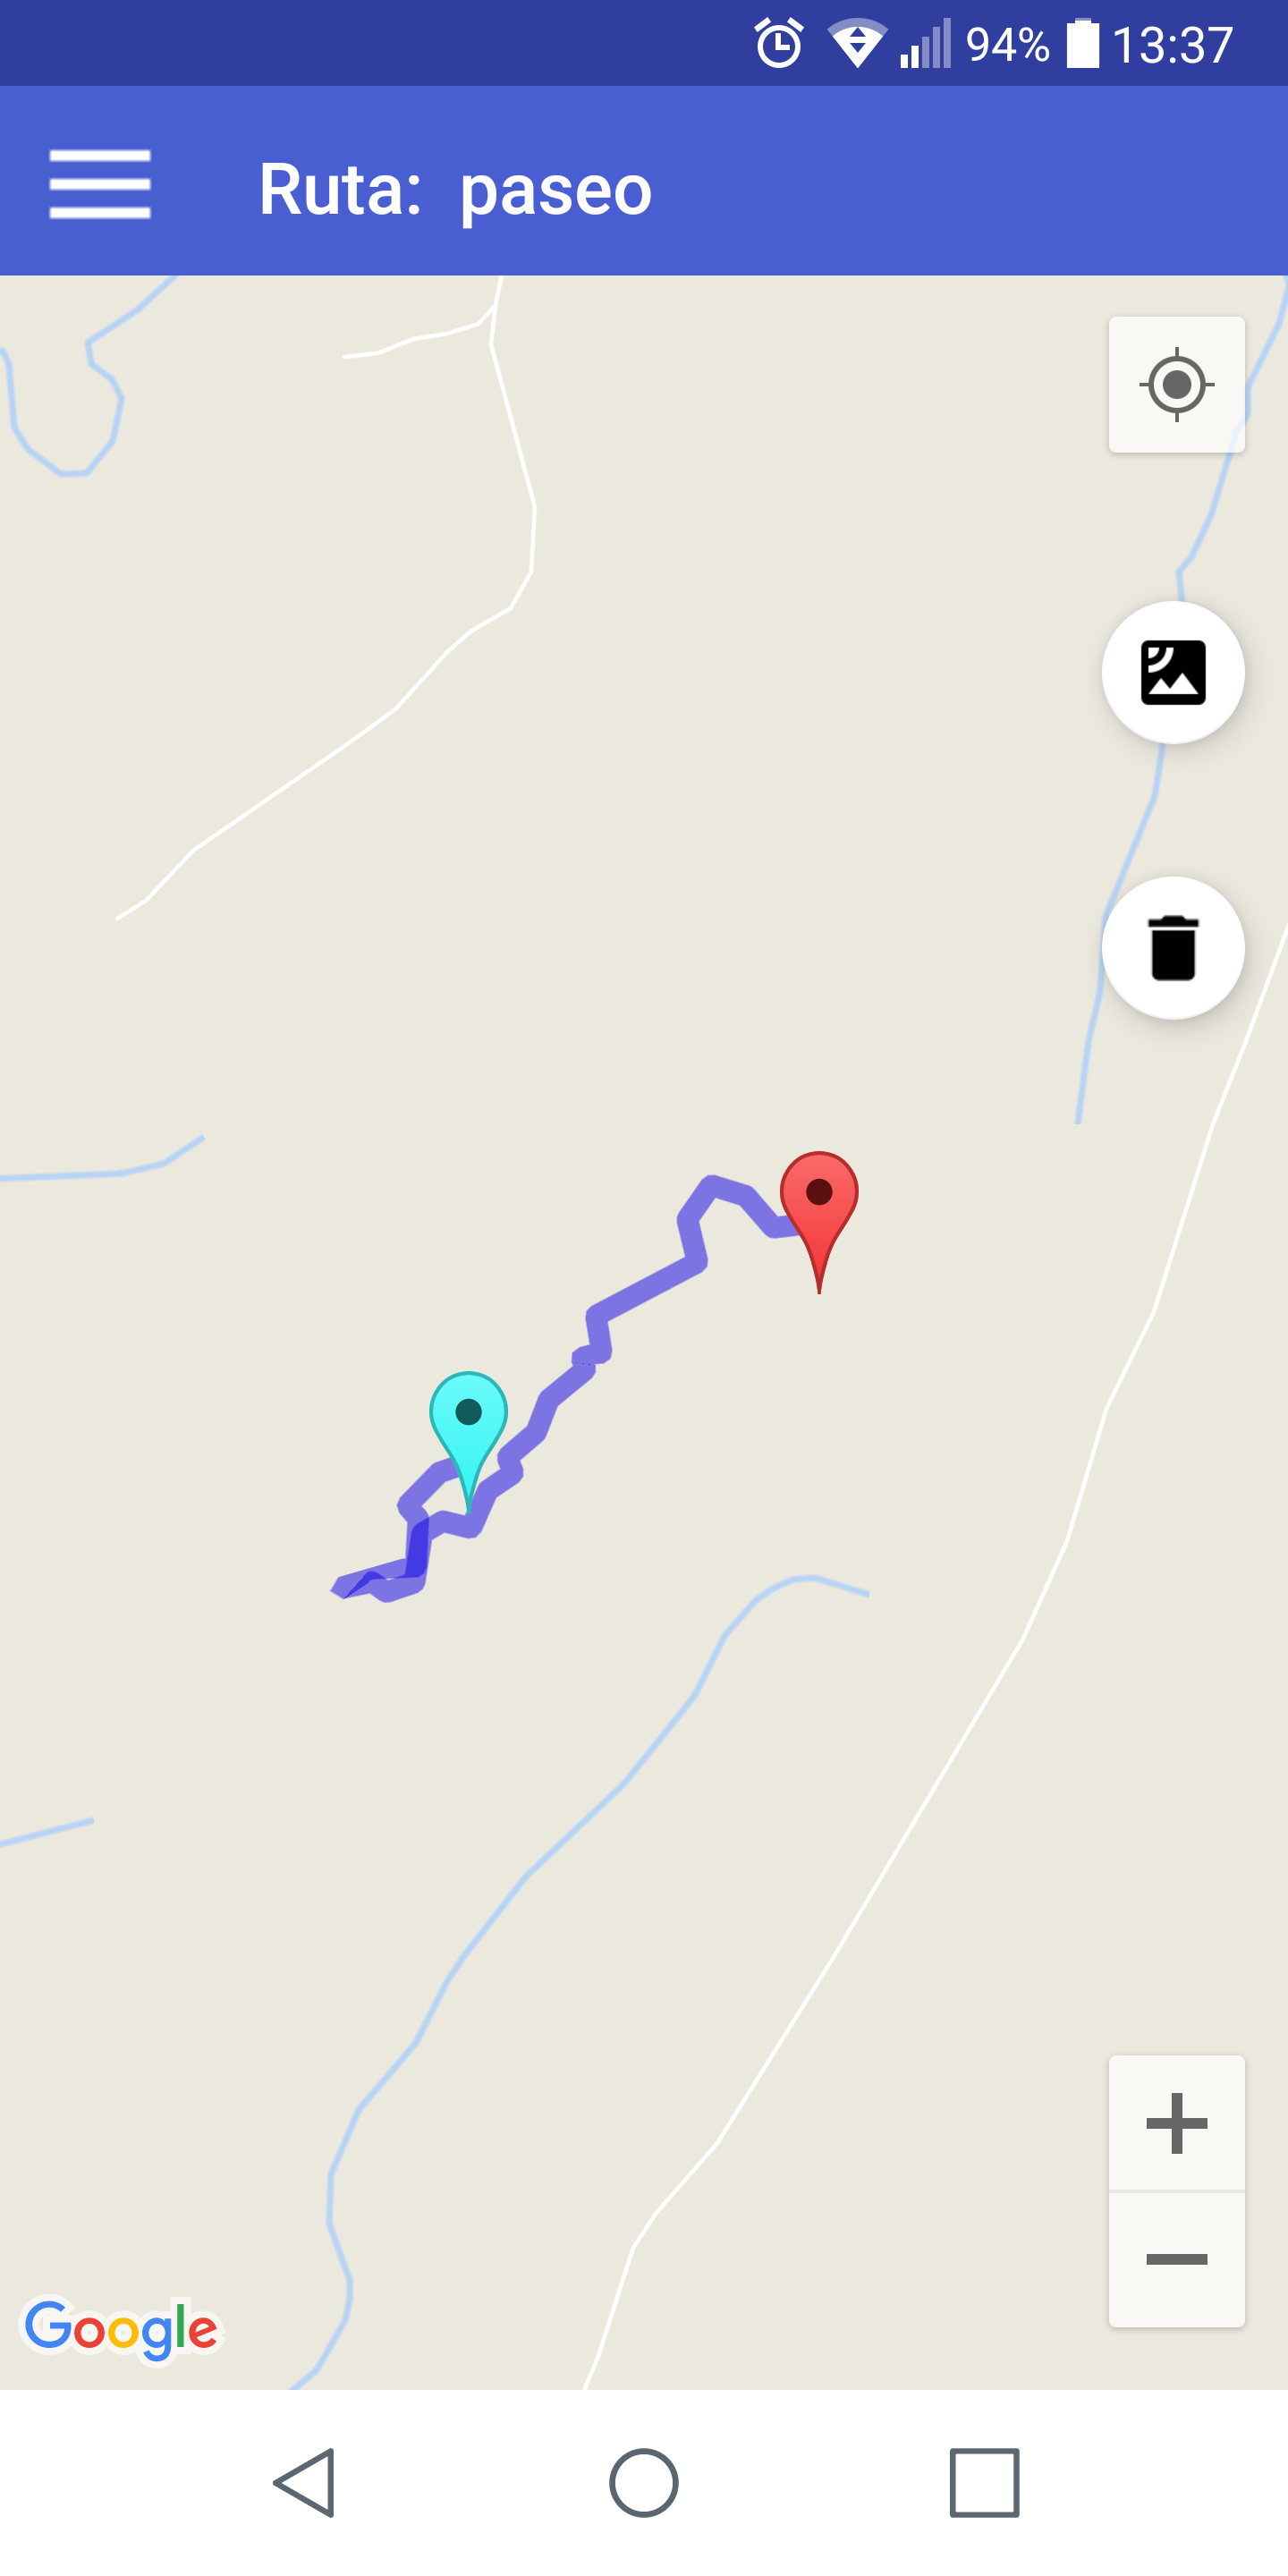
\includegraphics[width=6cm]{capturamovil/verruta1.png}
 \label{figura1}
\caption{Ruta seguida vista gráfica}

\end{minipage}
\hspace{0.5cm} % Si queremos tener un poco de espacio entre las dos figuras
\begin{minipage}[b]{0.5\linewidth}
\centering
\includegraphics[width=6cm]{capturamovil/verruta2.png}
 \label{figura2}
\caption{Ruta seguida vista satélite  }

\end{minipage}
\end{figure}


\begin{figure}[H]
		\centering
		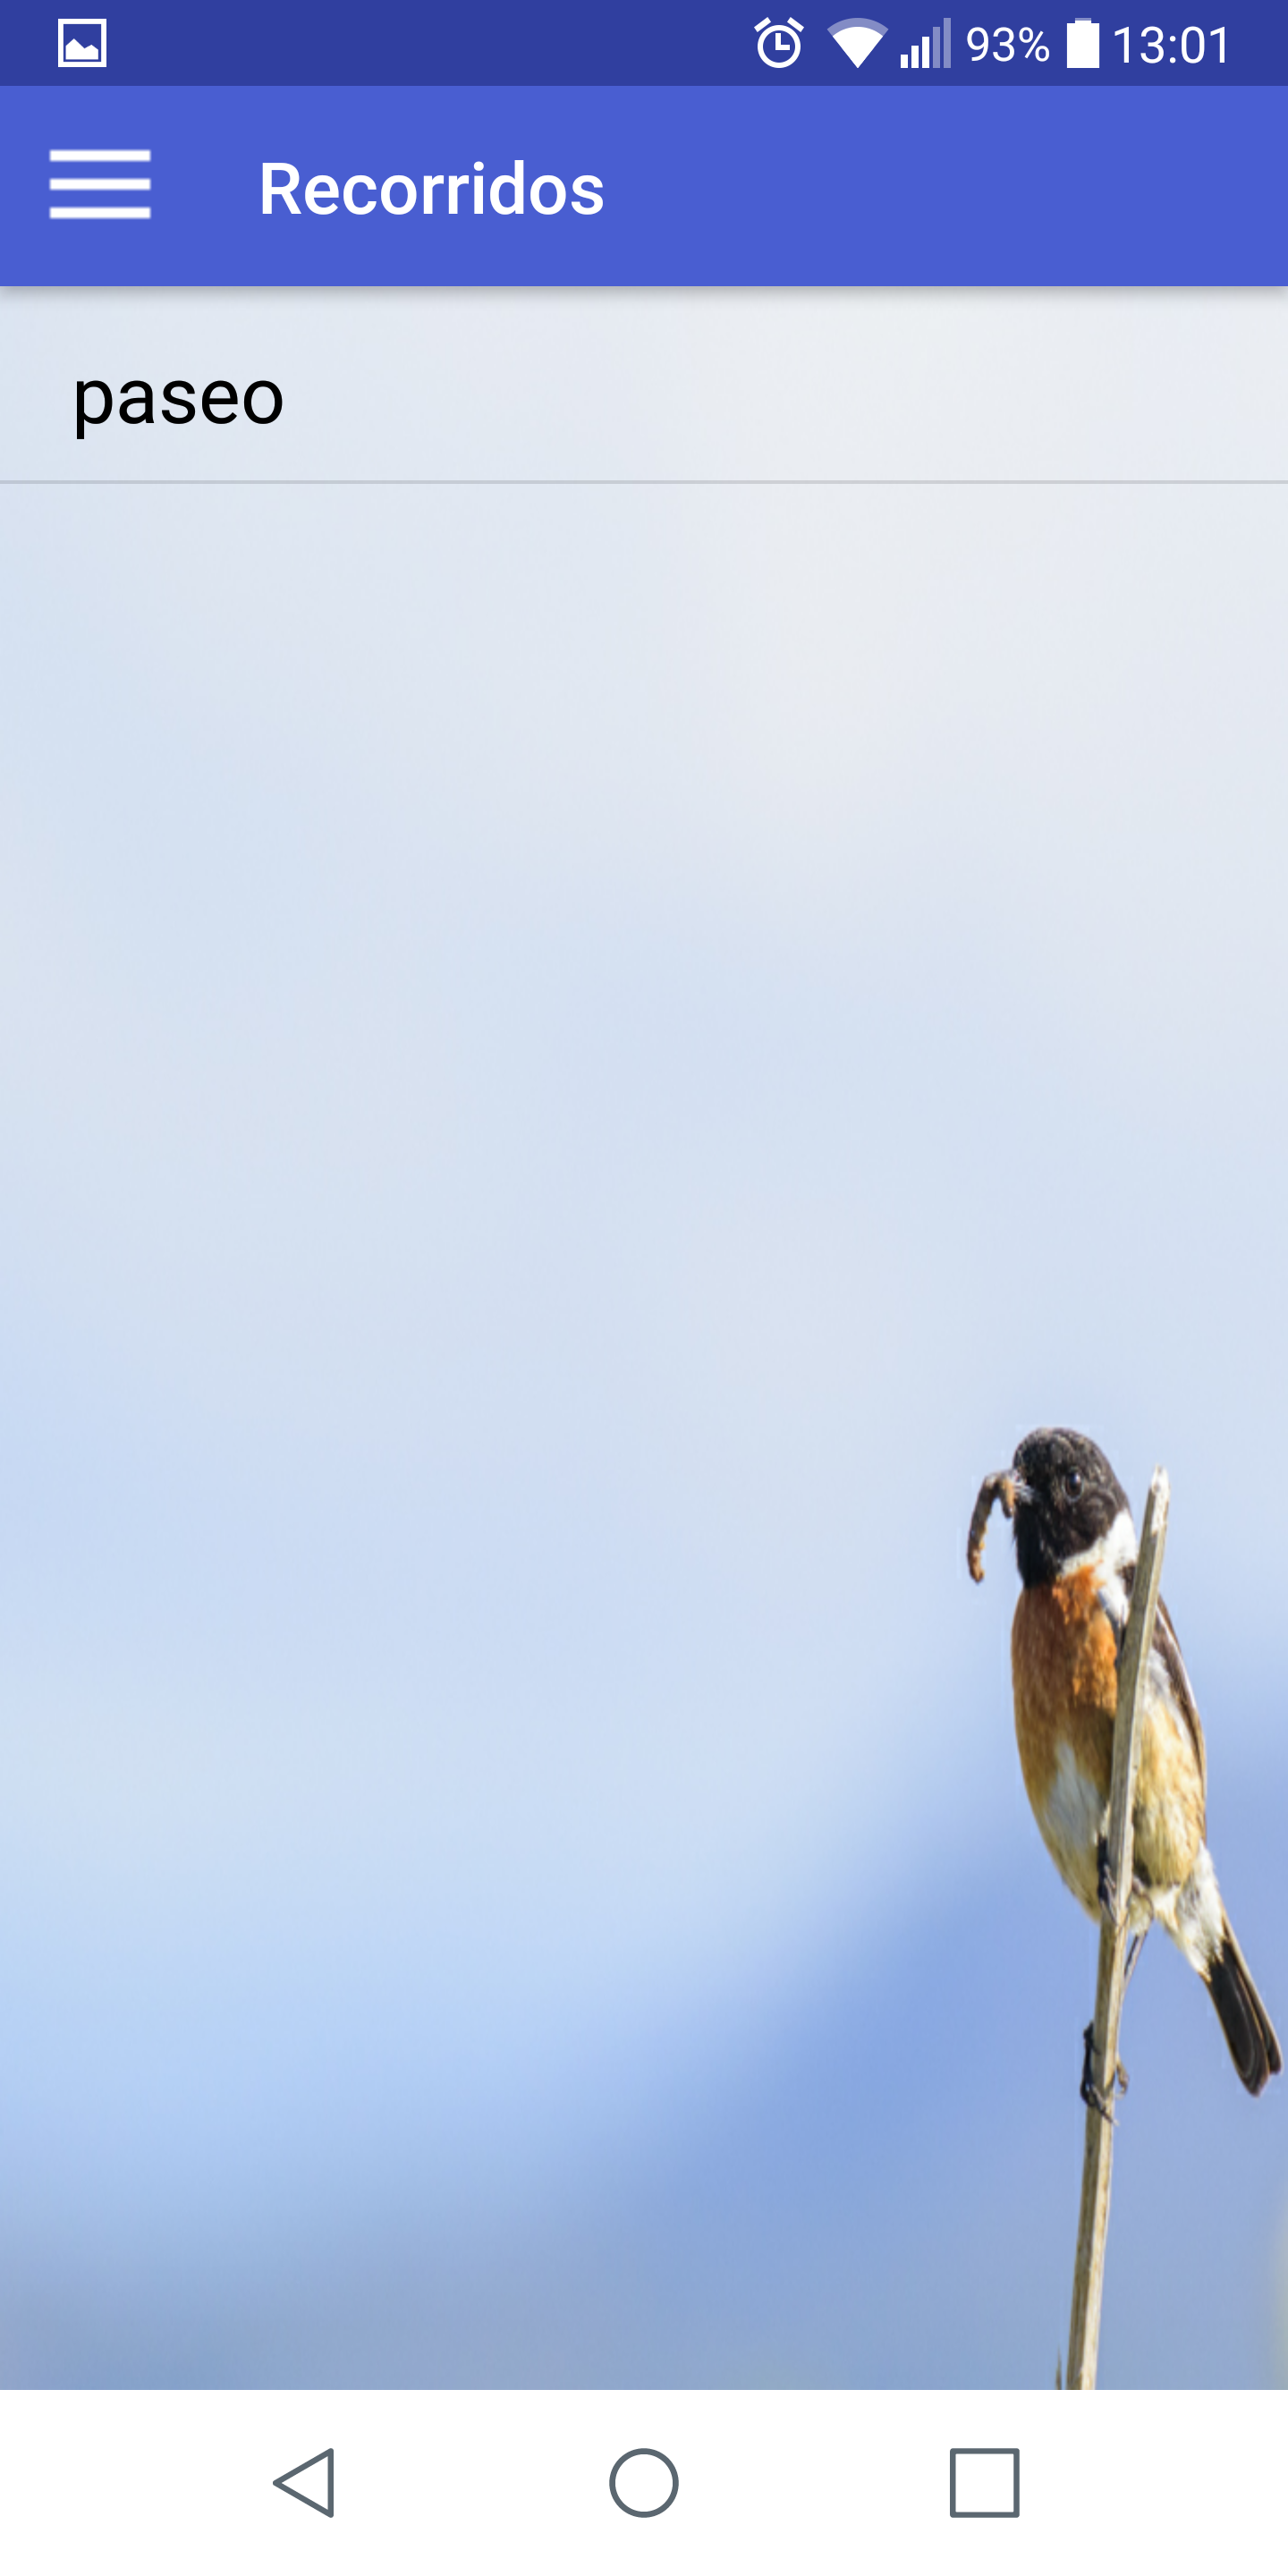
\includegraphics[width=0.3\textwidth] {capturamovil/listarutas}
		\caption{Lista de rutas creadas}
	\end{figure}

\subsection{Sprint 7}
Este Sprint contiene la historia más compleja de todas,\textbf{ \textit{gestionar una ruta compartida}}.

\begin{itemize}
\item \textbf{\textit{R-R-2 Crear ruta compartida}}
\item \textbf{\textit{R-R-2.1 Iniciar ruta}}
\item \textbf{\textit{R-R-2.2 Parar ruta}}
\item \textbf{\textit{R-R-2.3 Finalizar ruta}}
\end{itemize}

\subsection{Sprint 8}

Por ultimo en este Sprint se realizaran las pruebas finales, cierre del proyecto y la redacción de la memoria.

